\documentclass[11pt,twocolumn,notitlepage,openany,twoside]{book}
\usepackage[paperheight=11.25in,paperwidth=8.75in, margin=0.625in]{geometry}
\usepackage{titlesec}
\usepackage{verbatim}
\pagestyle{headings}

% Figure setup
\usepackage[]{graphicx}
\graphicspath{ {figures/} }
\usepackage{float}
\setlength{\floatsep}{0pt plus 2.0pt minus 2.0pt}
\setlength{\dbltextfloatsep}{5pt plus 2.0pt minus 2.0pt}
\usepackage{caption}
\captionsetup[figure]{font=small}

% % Table setup
% \usepackage[table]{xcolor}
% \usepackage{array}
% \newcolumntype{L}[1]{>{\raggedright\let\newline\\\arraybackslash\hspace{0pt}}m{#1}}
% \usepackage{multirow}
%
% \newcommand*{\tabbox}[2][t]{%
%     \vspace{0pt}\parbox[#1][1.7\baselineskip]{8pt}{\strut#2\strut}}
%
% \newcommand*{\tabboxb}[2][t]{%
%     \vspace{0pt}\parbox[#1][2.2\baselineskip]{8pt}{\strut#2\strut}}

% Remove the giant space at the beginning of a chapter
\titleformat{\chapter}[display]
    {\normalfont\huge\bfseries}{\chaptertitlename\ \thechapter}{20pt}{\Huge}
\titlespacing*{\chapter}{0pt}{0pt}{20pt}

\title{Metabolic interactions and capabilities within microbial communities}
\author{Gregory Leonard Medlock}


% % Optimization problem formatting
% \usepackage{amsmath}
%
% % Bibliography setup
% \usepackage[backend=biber, style=numeric-comp,sorting=none,terseinits=true, giveninits=true,maxbibnames=4]{biblatex}
% \addbibresource{rf_references.bib}
% \DeclareNameAlias{default}{last-first}
% \renewcommand*{\revsdnamepunct}{}
% \renewcommand*{\bibfont}{\small}

\usepackage[backend=biber, style=numeric-comp,sorting=none,terseinits=true, giveninits=true,maxbibnames=4]{biblatex}
\addbibresource{rf_compiled_refs.bib}
% There's a non-ASCII character somewhere in the bib, so we need this package:
\usepackage[utf8]{inputenc}

\begin{document}
\frontmatter

\begingroup
\let\clearpage

\setcounter{tocdepth}{3}
\tableofcontents
\hspace{1.5cm}
\listoffigures
\hspace{1.5cm}
\listoftables

\endgroup

\clearpage
\addcontentsline{toc}{chapter}{Acknowledgments}
\section*{Acknowledgments}

Acknowledgements will be here

\mainmatter


%------------------------------------------------------------------------------------
% Chapter 1 Introduction
%------------------------------------------------------------------------------------
\chapter{Introduction}
\begin{refsection}

\section{Specific Aims}

These the aims:

\begin{enumerate}
  \item \textbf{Aim 1: Identify \textit{in vitro} metabolic interactions between members of a defined mouse microbiota}. Aim 1
  \item \textbf{Aim 2: Develop an ensemble-driven framework for the refinement and application of genome-scale metabolic network reconstructions of gut microbes}. Aim 2
\end{enumerate}



\section{A Preview of this Dissertation}

Preview text\cite{Song2005-mt}
\section{References}

\printbibliography[heading=none]
\end{refsection}

%------------------------------------------------------------------------------------
% Chapter 2
%------------------------------------------------------------------------------------
\chapter{Inferring Metabolic Mechanisms of Interactions within a Defined Gut Microbiota}
\chaptermark{Metabolic interactions}

\begin{refsection}

The contents of this chapter are published as a research article here:

\medskip\noindent
Medlock GL, MA Carey, DG McDuffie, MB Mundy, N Giallourou, JR Swann, GL Kolling, JA Papin. (2018). Inferring Metabolic Mechanisms of Interactions within a Defined Gut Microbiota. \textit{Cell Systems}, 7(3):p245-357.e7.

\section{Context}

\section{Synopsis}

The diversity and number of species present within microbial communities create the potential for a multitude of interspecies metabolic interactions. Here, we develop, apply, and experimentally test a framework for inferring metabolic mechanisms associated with interspecies interactions. We perform pairwise growth and metabolome profiling of co-cultures of strains from a model mouse microbiota. We then apply our framework to dissect emergent metabolic behaviors that occur in co-culture. Based on one of the inferences from this framework, we identify and interrogate an amino acid cross-feeding interaction and validate that the proposed interaction leads to a growth benefit \textit{in vitro}. Our results reveal the type and extent of emergent metabolic behavior in microbial communities composed of gut microbes. We focus on growth-modulating interactions, but the framework can be applied to interspecies interactions that modulate any phenotype of interest within microbial communities.

\section{Introduction}

The structure and function of microbial communities may influence human health through a variety of means \cite{Turnbaugh2007-cd}. However, understanding the mechanisms governing this influence is complicated by the complexity of microbial communities. Interspecies interactions within microbial communities underlie benefits to human health, such as colonization resistance to pathogens \cite{Britton2014-wm, Buffie2013-xt}. These interspecies interactions are often metabolic, such as competition for metabolites essential for growth of pathogens \cite{Gillis2018-mt,Lawley2013-ez,Stecher2008-bc}. Since metabolic interactions occur between distantly-\cite{Fischbach2011-wg} and closely-related \cite{Rakoff-Nahoum2014-dw} species, creating heuristics for identifying presence or absence of interactions based on phylogeny is challenging.

Knowledge of interactions among small subsets of community members has been shown to enable prediction of community assembly in larger communities, suggesting that constructing predictive models of population dynamics in complex microbial communities may be a tractable problem \cite{Friedman2017-zn}. However, in this same study, while pairwise interactions were sufficient to predict community assembly in 3-species pairs, information from 3-species communities was necessary to predict assembly of larger communities. Further supporting the lack of generalizability of pairwise interactions to new conditions, theoretical ecological analyses suggest that universal interspecies interaction terms in pairwise ecological interaction models cannot recapitulate commonly identified chemical-mediated interspecies interactions \cite{Momeni2017-it}. Thus, generalizable methods for predicting assembly of large microbial communities likely depend on more mechanistic knowledge of interactions that can help account for context specificity, such as the consumption and production of metabolites that might be shared within a community \cite{Goldford2017-zx}.

The spatial, temporal, and compositional complexity of microbial communities in mammals make inferring mechanisms of interaction challenging. Using gnotobiotic animals can improve the tractability of this problem. However, knowledge of the behavior of individual microbes within the defined community is generally lacking unless classical model organisms are used in place of naturally occurring organisms. To increase the value of experiments performed using gnotobiotic animals, individual members of the microbiota can be characterized in vitro. The phenotyping performed via these experiments improves our understanding of these organisms, which may improve our ability to predict and interpret how they might behave in vivo.

\begin{figure*}[tb]
\centering
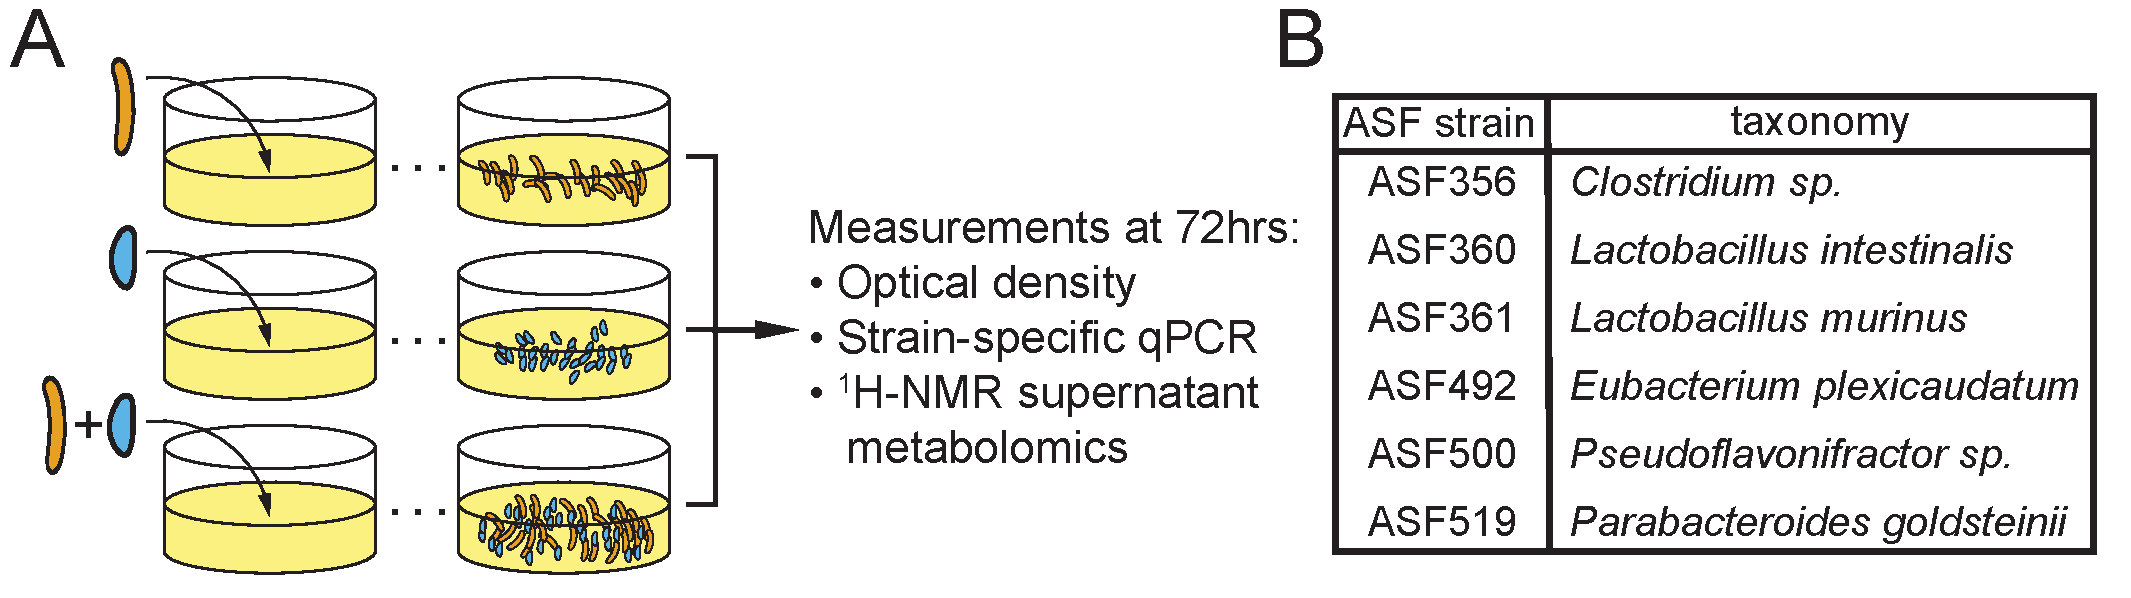
\includegraphics[width=0.8\textwidth]{ch2_fig1}
\caption[Summary of co-culture experiment design, measurements, and total growth outcomes in monocultures and co-cultures.]{\textbf{Summary of co-culture experiment design, measurements, and total growth outcomes in monocultures and co-cultures.} \textbf{A)} Experimental procedure for each pair of strains and measurements taken. \textbf{B)} Taxonomic assignment for strains included in this study.}
\end{figure*}

The altered Schaedler flora (ASF) is a group of 8 bacterial strains isolated from the mouse gastrointestinal tract used to standardize the microbiota of laboratory mice \cite{Wymore_Brand2015-ez}. ASF-colonized mice remain stably colonized across mouse generations and have normalized organ physiology relative to germ-free mice \cite{Wymore_Brand2015-ez}. Although there are known differences between the immune repertoires of ASF-colonized mice and conventional mice, these differences can be exploited to test specific hypotheses \cite{Geuking2011-fj,Ivanov2009-vl}. ASF mice have been used widely in infectious disease research to study Clostridium difficile \cite{Schwan2009-zo}, Salmonella enterica \cite{Brugiroux2016-vi}, and Cryptosporidium parvum \cite{Harp1992-wr}. Many specific pathogen-free mice are initially colonized with the ASF, which has led to the theory that presence or absence of ASF strains contributes to vendor-specific differences in susceptibility to disease \cite{Singer2000-tr}.  Further use of gnotobiotic systems such as ASF-colonized mice could greatly accelerate discovery in microbiome research, especially if the behavior of the ASF alone is well-understood.

Previously, we performed pairwise spent media experiments using seven of the ASF strains, in which each strain was grown in the same medium as well as the spent medium of other strains \cite{Biggs2017-fs}. We identified cases of putative cross-feeding and competition and the effect of those interactions on growth dynamics. However, each strain was spatially and temporally separated in that study. While spent media experiments remove some technical and statistical complications in inferring metabolic interactions, the interactions that are possible are different than those that might occur while strains are grown in co-culture.

Here, we further define the interactive potential of six of the ASF strains and develop an analytic method to infer putative mechanisms of metabolic interaction. We perform co-culture growth experiments with all pairs of these strains and profile their supernatant metabolomes in both mono- and co-culture. We identify the influence of interspecies interactions on growth of each strain, then apply our analytic framework for inferring putative metabolic mechanisms of interaction from supernatant metabolomic data. We experimentally interrogate an inferred cross-feeding interaction in which one ASF strain (Parabacteroides goldsteineii ASF519) produces amino acids that another (Clostridium sp. ASF356) consumes, confirming that the hypothesized mechanism occurs and leads to a growth benefit for the consuming strain. With this new insight, we provide a framework to identify putative metabolic mechanisms of microbe-microbe and host-microbe interactions that can be applied to any microbial community to investigate co-culture phenotypes including growth enhancement or changes in metabolite yield.

\section{Results}
\subsubsection{Ecological interactions within the altered Schaedler flora}

We collected \textit{in vitro} data for growth of all pairwise combinations of 6 ASF strains (Figure 2.1A, n=6-9 per strain pairing). Taxonomic assignments for these strains are provided in Figure 2.1B. We determined the impact of co-culture on each strains’ growth by comparing monoculture abundance after 72 hours of growth to the abundance of each strain in co-culture at the same time (determined using probe-based qPCR; all strains are in stationary phase; see example growth curves in Figure S2.2; see Methods).

\begin{figure*}
\centering
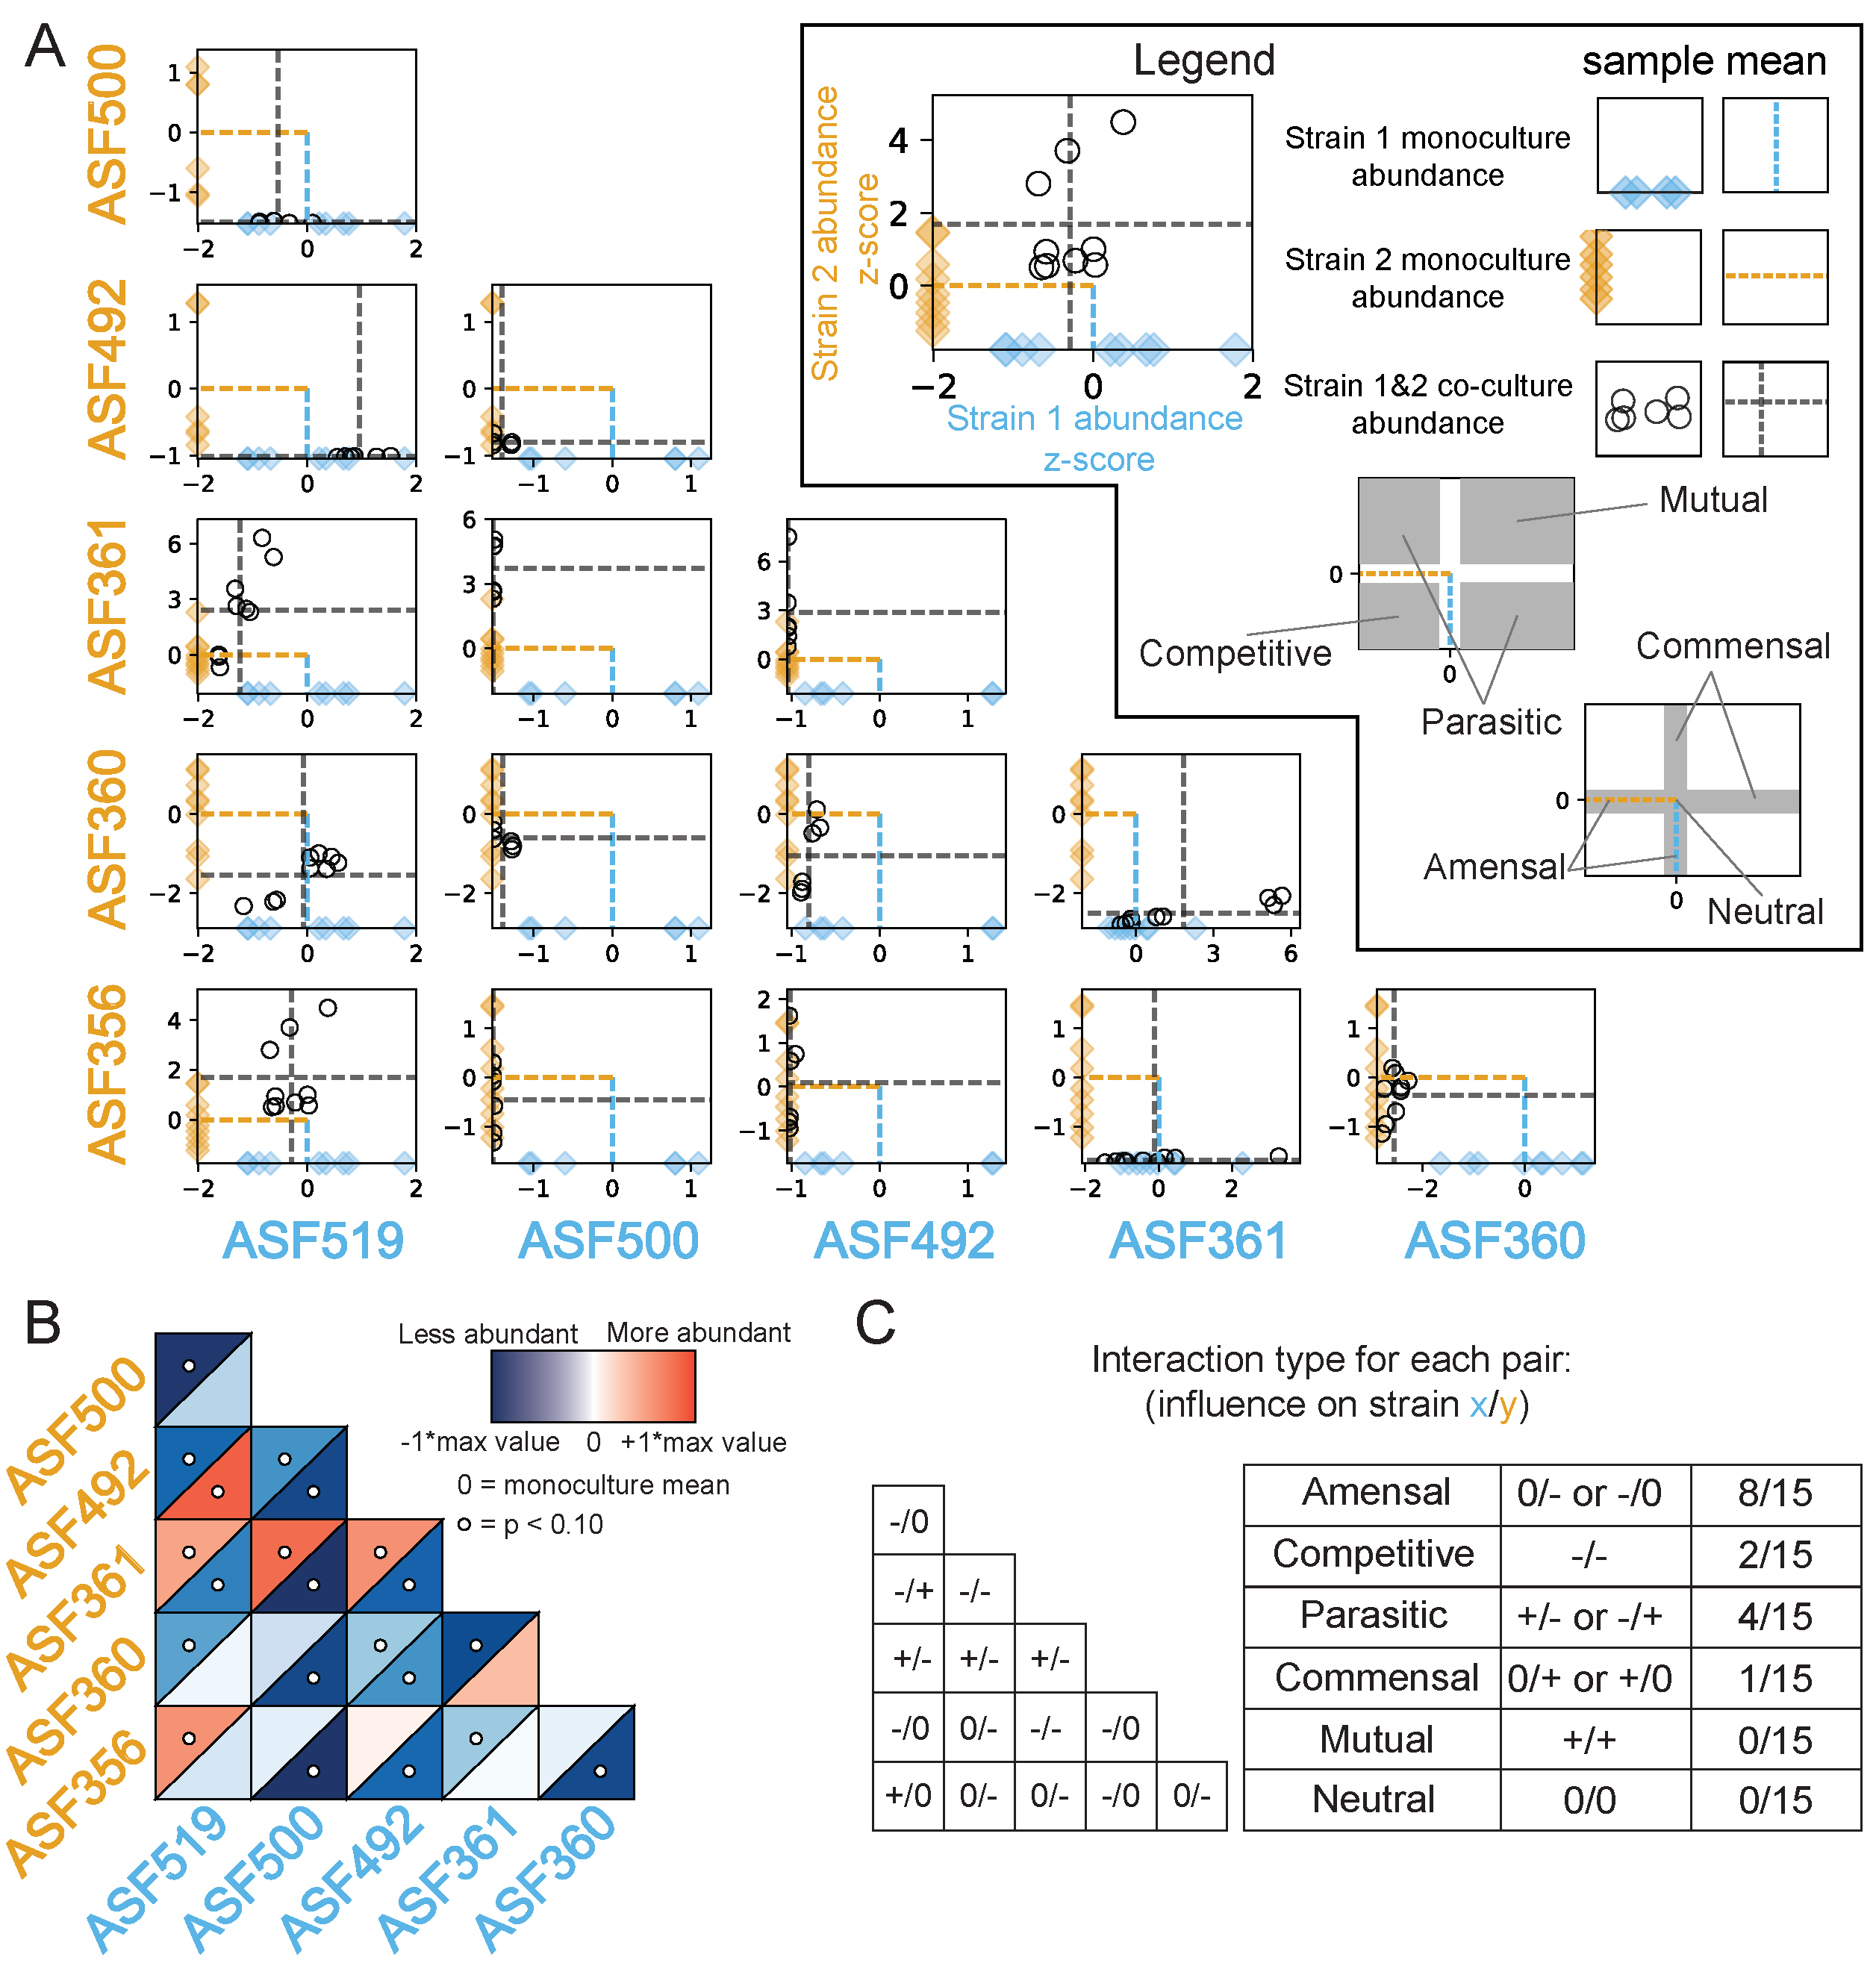
\includegraphics[width=0.9\textwidth]{ch2_fig2}
\caption[The effects of pairwise co-culture on the abundance of each strain.]{\textbf{The effects of pairwise co-culture on the abundance of each strain.} \textbf{A)} Relative abundance of each strain in monoculture and co-culture determined via qPCR. Abundance is plotted on linear scale, not log-transformed. x-axis describes abundance of strain at the bottom of the column; y-axis describes abundance of strain left of each row. Diamonds indicate abundance of each strain in monoculture, with mean shown by a dashed line. Abundance of each strain in co-culture as indicated by the row and column labels is shown by a black circle, with mean abundances indicated by grey dashed lines. Abundance for each strain is z-score normalized using mean and standard deviation of monoculture abundance to center and scale the data, respectively. N=9 for all samples except for those with Pseudoflavonifractor ASF500 or Eubacterium ASF492, for which N=6. \textbf{B)} Heatmap of mean abundance of each strain in co-culture relative to monoculture. Blue indicates less abundant, while red indicates more abundant, than monoculture. The upper left and lower right triangles in each square describes abundance of the strain labelled on the left of row and bottom of column, respectively. White circles indicate differential abundance between monoculture and co-culture (\textit{p} < 0.10, Mann-Whitney U test with false discovery rate correction using Benjamini-Hochberg procedure). \textbf{C)} Summary of interspecies interactions. Non-zero interactions in the triangular matrix indicate significant differential abundance as shown in Figure 2B.}
\end{figure*}

Abundance of each strain in each pair was evaluated to determine whether a negative (-), positive (+), or neutral (0) effect on abundance occurred in the pairing, allowing classification of pairwise interaction with standard ecological terminology. All pairings except one, \textit{Clostridium} ASF356 with \textit{Parabacteroides} ASF519, had a negative impact on the abundance of at least one strain, with 0/- (amensalism), +/- (parasitism), -/- (competition), and +/0 (commensalism) being the only interactions detected (8, 4, 2, and 1 instances, respectively; data shown in Figure 2.2A, summarized in Figure 2.2B and 2.2C). \textit{Lactobacillus} ASF361 was present in 3/4 parasitic co-cultures and experienced a growth benefit in all cases. In contrast, growth of both \textit{Eubacterium} ASF492 and \textit{Pseudoflavonifractor} ASF500 was inhibited in every condition, including in co-culture with each other. In summary, abundance of individual strains tended to be lower in co-culture than in monoculture. However, the growth benefit observed for some strains also suggests that differences in resource utilization across strains, or emergent behavior in co-culture such as cross-feeding and consumption of novel substrates/metabolites, occurred in some co-cultures.

\subsubsection{Metabolic repertoires within the altered Schaedler flora}

\begin{figure*}[t]
\centering
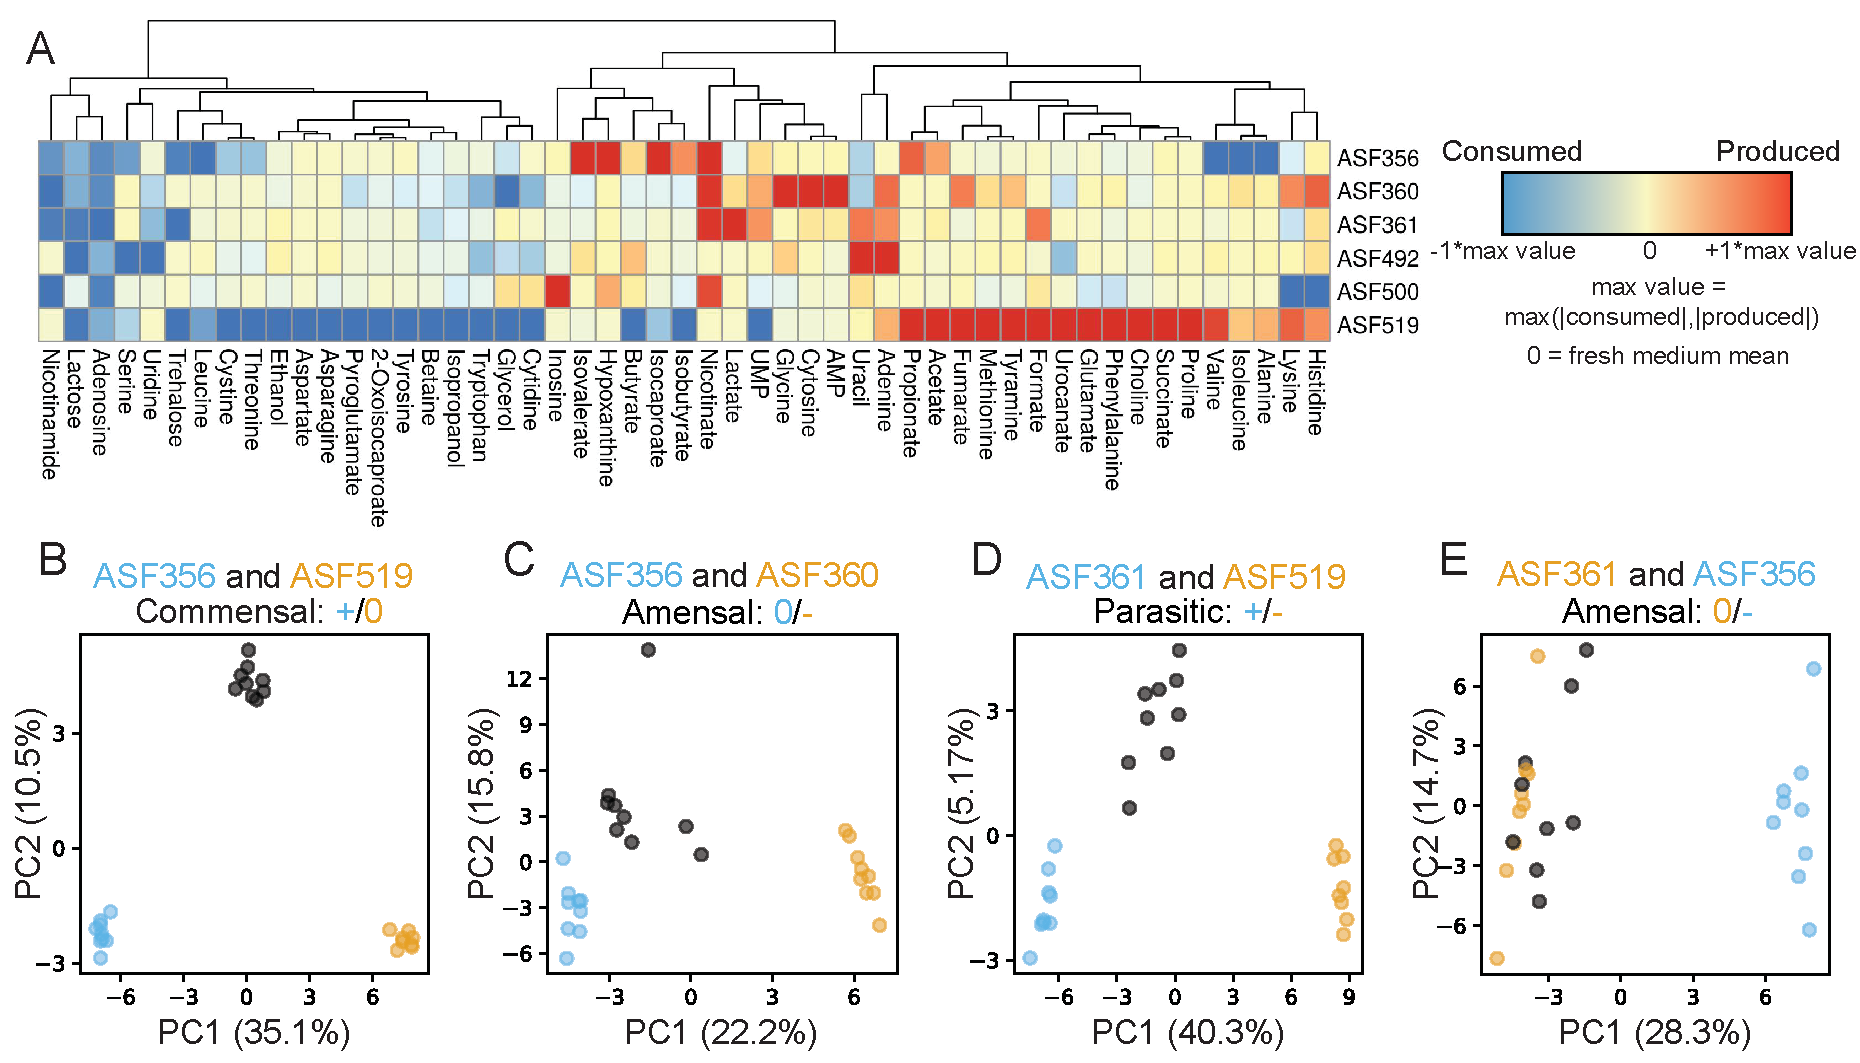
\includegraphics[width=0.8\textwidth]{ch2_fig3}
\caption[Metabolic behavior of each strain in monoculture and emergent behavior in co-cultures.]{\textbf{Metabolic behavior of each strain in monoculture and emergent behavior in co-cultures.} \textbf{A)} Heatmap describing supernatant metabolomes for each monoculture. Red/blue indicate higher/lower concentrations than fresh medium, respectively. Values are centered at 0 using the mean in fresh media, then scaled between -1 and +1 by dividing by the maximum change in concentration for each metabolite in any sample in the study. Unnamed metabolites not shown. Hierarchical clustering was performed using Euclidean distances and complete linkage. \textbf{B-E)} Principal component analysis (PCA) of monocultures and co-culture, performed independently for each subplot. Sky blue/orange circles correspond to monoculture supernatant metabolomes from strain labelled with same color. Co-culture samples for the two strains in each subplot title are indicated by grey circles. Percent variance captured by each principal component is labelled on each axis.}
\end{figure*}

To determine potential mechanisms governing the changes in growth observed in co-culture, we performed metabolomics on the spent supernatant from all samples in the growth experiments (using  $^1\!$H NMR spectroscopy, see Methods). We updated and refined the metabolite peak annotations from experiments previously performed using the same medium and strains \cite{Biggs2017-fs}, resulting in 86 detected metabolites, 50 of which could be assigned an identity (36 of 85 metabolites were previously assigned an identity). We identified new metabolites involved in amino acid metabolism (serine, cystine, asparagine, glutamate, 2-oxoisocaproate, and isocaproate), nucleic acid metabolism (cytidine, cytosine, uridine monophosphate), and anaerobe-specific metabolism (isopropanol).

Based on the monoculture supernatant metabolomic profiles presented here (Figure 2.3A) and in our previous study of the ASF, the ASF strains have fermentation repertoires similar to closely-related gut microbes \cite{Biggs2017-fs}. \textit{Lactobacillus} ASF360 and \textit{Lactobacillus} ASF361 both produced lactate, while \textit{Lactobacillus} ASF361 also produced acetate and formate. Other strains of \textit{Lactobacillus intestinalis} and \textit{Lactobacillus murinus} are generally identified as facultative heterofermentative lactic acid bacteria \cite{Vos2011-bf}. Heterofermentative lactic acid bacteria ferment carbohydrates to lactate but may also produce additional acetate in some conditions. \textit{Clostridium} ASF356 produced the common fermentation end products acetate, propionate, succinate, and butyrate. Butyrate production is common in \textit{Clostridia} that inhabit mammalian gastrointestinal tracts, and is often coupled with acetate production \cite{Louis2009-ax}. Propionate is the primary end product of three common pathways identified in anaerobic organisms, of which the acrylate pathway and succinate pathway have been identified in \textit{Clostridia spp.} \cite{Reichardt2014-ua}. \textit{Clostridium} ASF356 also produced isovalerate, isocaproate, and isobutyrate, which are common products of amino acid fermentation by some \textit{Clostridia spp.} \cite{Mead1971-oa}.

Butyrate and ethanol were the only common fermentation end products produced by \textit{Eubacterium} ASF492. \textit{Eubacterium} ASF492 has been proposed as the type strain for \textit{Eubacterium plexicaudatum} \cite{Dewhirst1999-pp}, which was originally identified as producing butyrate and small amounts of acetate from glucose \cite{Wilkins1974-yn}. \textit{Pseudoflavonifractor} ASF500 produced only formate and consumed less lactose than any other ASF strain, suggesting that lactose is not a preferred carbon source for \textit{Pseudoflavonifractor} ASF500 or another growth-limiting nutrient is only present at low abundance in the medium. \textit{Parabacteroides} ASF519 produced acetate, propionate, and succinate, consistent with previous reports on fermentation products of \textit{Parabacteroides goldsteinii} \cite{Song2005-mt}, as well as formate. \textit{Parabacteroides} ASF519 also produced many amino acids, including histidine, lysine, alanine, isoleucine, valine, proline, phenylalanine, glutamate, and methionine, suggesting \textit{Parabacteroides} ASF519 contains a comprehensive amino acid biosynthesis repertoire.

\subsubsection{Co-culture can lead to emergent metabolic behavior}

Co-culture substantially altered the metabolome of pairings relative to each of the monoculture metabolomes for the strains involved (see Figure S1 for results from all groups). To detect and quantify the emergent metabolic behavior resulting from co-culture, we performed principal component analysis (PCA; see Methods) on the metabolic profile for pairs of strains. We performed PCA separately for each pair of strains, including samples from each monoculture and the co-culture. In cases where both strains grew in co-culture (i.e. no strong negative growth effect), the first principal component (PC1) separated monocultures by strain and the second principal component (PC2) separated monoculture samples from co-culture samples. This behavior was particularly strong in the case of \textit{Clostridium} ASF356 and \textit{Parabacteroides} ASF519 (Figure 2.3B). For \textit{Clostridium ASF356} and \textit{Parabacteroides} ASF519, the loadings of PC2 suggest that co-culture increased production of propionate, glycine, and the amino acid fermentation products isovalerate, isocaproate, and isobutyrate, and increased consumption of multiple amino acids and lactose.

For pairings with a strong negative effect on one strain, the co-culture metabolomes were less similar to the negatively-affected strain than the other strain. For example, co-culture of \textit{Clostridium ASF356} with \textit{Lactobacillus} ASF360 resulted in decreased growth of \textit{Lactobacillus} ASF360, and the co-culture samples are located closer to \textit{Clostridium} ASF356 monoculture samples in PCA (Figure 2.3C). Although there is still an “emergent” co-culture effect observed in PC2 for this pair, the effect is also aligned with within-group variation. The same trend is present for \textit{Lactobacillus} ASF361, \textit{Parabacteroides} ASF519, and their co-culture (Figure 2.3D). For strong negative growth outcomes (e.g. \textit{Clostridium} ASF356 and \textit{Lactobacillus} ASF361 co-culture), the effect is more pronounced and there is less separation between monoculture and co-culture samples (Figure 2.3E).

\subsubsection{Development of an expectation-based model to account for changes in strain abundance}

Based on the metabolic differences between monoculture and co-culture samples identified via PCA, co-culture conditions substantially altered metabolic behavior. However, the mechanism that leads to this emergent metabolic behavior is unclear, and attempting to infer the mechanism may be confounded by changes in the abundance of each strain in co-culture. We sought to infer metabolic interactions between strains in co-culture by accounting for changes in strain abundance. While the absolute amount of a metabolite produced or consumed may change in co-culture relative to monoculture, taking changes in strain abundance into account is necessary to determine whether the change in metabolite abundance is emergent behavior rather than additive.

\begin{figure*}[tb!]
\centering
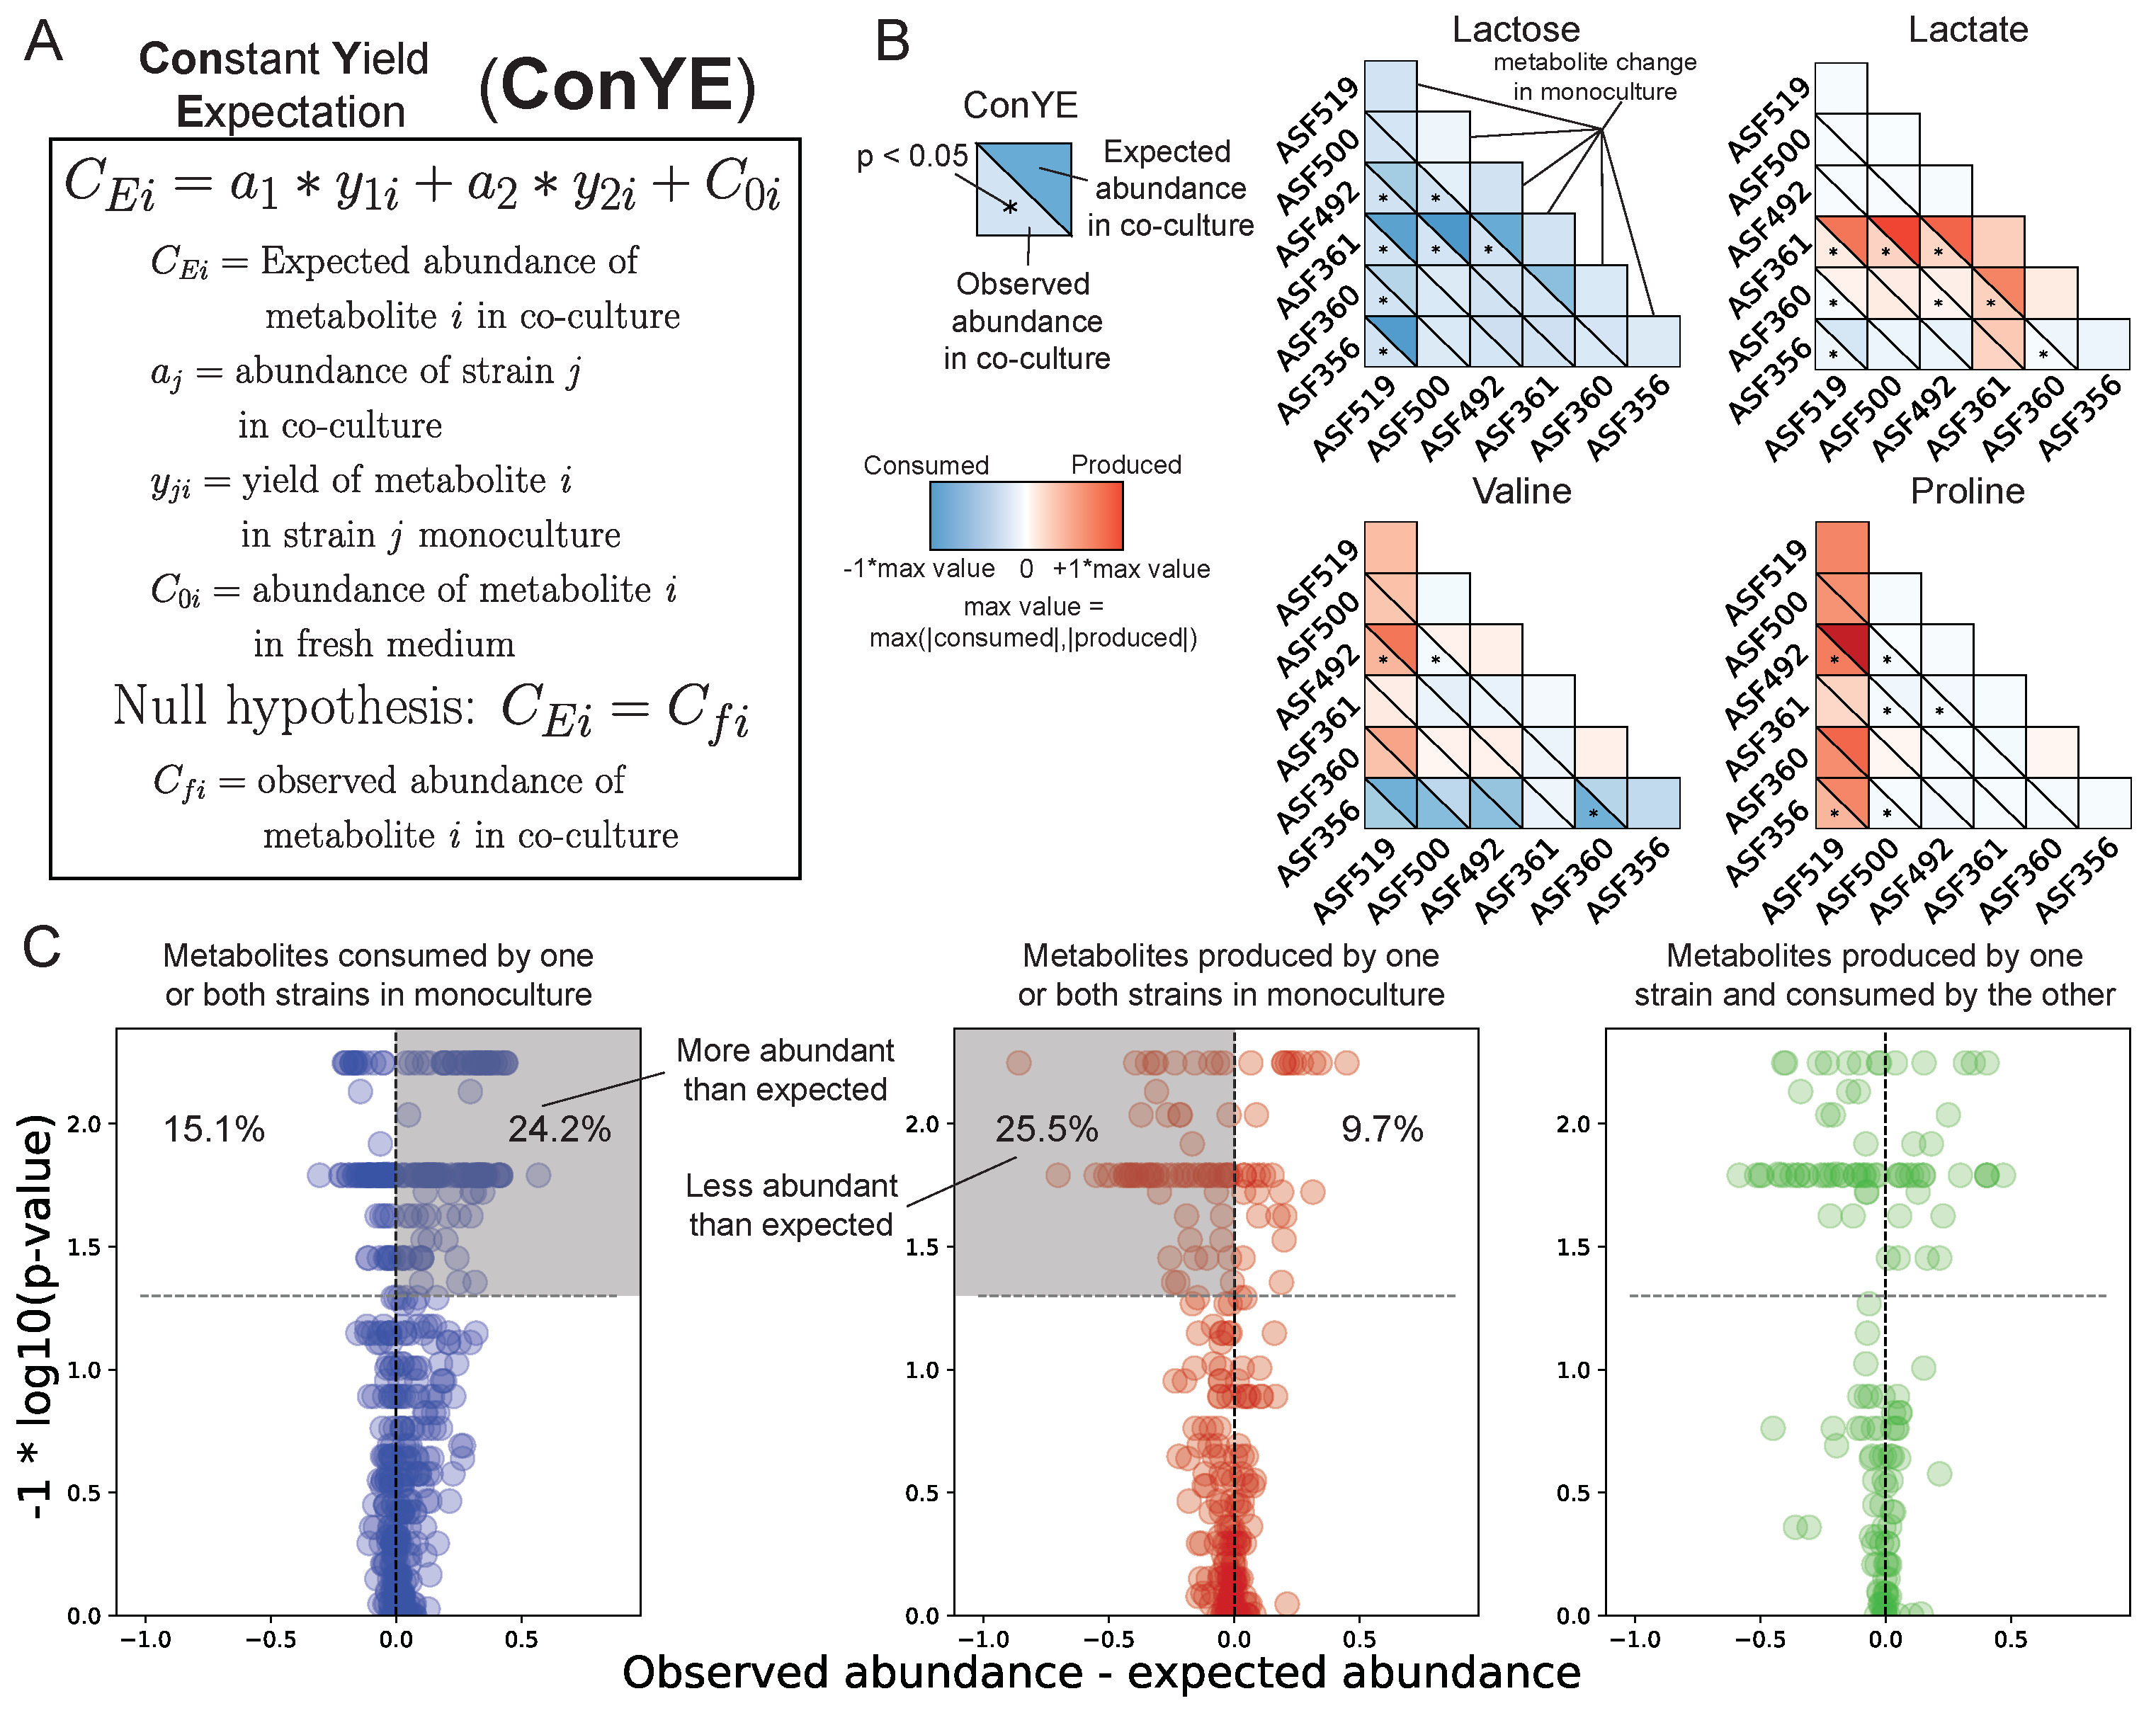
\includegraphics[width=0.9\textwidth]{ch2_fig4}
\caption[Accounting for co-culture growth outcomes with ConYE to identify emergent metabolism.]{\textbf{Accounting for co-culture growth outcomes with ConYE to identify emergent metabolism.} \textbf{A)} Procedure for the constant yield expectation (ConYE) model. \textbf{B)} Examples of ConYE results for Lactose, Lactate, Valine, and Proline. Diagonal shows monoculture behavior for each strain. Every pair of triangles indicates the observed metabolite abundance in co-culture (lower left), the expected metabolite abundance (upper right), and whether there was a significant difference between observed and expected values. Centering and scaling performed as in Figure 3, except expected values were included while selecting a max value. Mann-Whitney U-Test with false discovery rate (FDR) control using the Benjamini-Hochberg procedure was performed for all 1290 comparisons (15 co-cultures, 86 metabolites each). Asterisk indicates p < 0.05 for the metabolite in the co-culture containing the indicated strains. \textbf{C)} ConYE results for all strain pairings for metabolites that were consumed by one or both strains in monoculture (left, blue), produced by one or both strains in monoculture (middle, red), or produced by one strain in monoculture and consumed by the other strain in monoculture (right, green). Each point represents a metabolite in a co-culture pair. x axis show the difference between observed and expected metabolite abundance in co-culture (scaled as in panel B), and y axis shows the p-value from ConYE. Points above grey line have p < 0.05. Percentage of points in the labelled quadrant relative to the rest of the points in the subplot is shown.}
\end{figure*}

We developed a Constant Yield Expectation (ConYE) model to identify metabolites for which consumption or production behavior changed in co-culture (see Methods). Within the ConYE model, we assume each strain produces or consumes a fixed quantity of each metabolite per unit biomass (i.e. constant yield), then test whether that assumption is true in co-culture by comparing the expected behavior to the observed co-culture data. We simulate expected metabolite quantities in co-culture by multiplying the mono-culture-derived metabolite yield for each strain by the observed abundance of that strain in co-culture, then summing the expected values for each strain and the initial quantity of the metabolite present in the fresh medium (Figure 2.4A). For each metabolite, we test the null hypothesis that the quantity of that metabolite in co-culture is equal to that predicted by the ConYE model. Rejecting the null hypothesis for a metabolite implies that co-culture caused at least one strain to alter metabolism of that metabolite relative to its own biomass production.

We identified several patterns with the ConYE model results that were consistent across sets of many metabolites, for which representative examples are shown (Figure 2.4B). Metabolites consumed in monoculture were often consumed less than expected in co-culture, especially when one strain in the co-culture experienced a growth benefit (e.g. lactose). For some strains, this pattern may arise because alternative metabolites are now available in co-culture that can be consumed to produce biomass, decreasing the amount of lactose required to produce a unit of biomass. Similarly, another pattern involves fermentation end products, which were generally less abundant than expected. Lactate, which was produced by \textit{Lactobacillus} ASF360 and \textit{Lactobacillus} ASF361, was less abundant than expected in 7/9 co-cultures containing either strain. Explanations for this pattern align with explanations for the first pattern; individual strains may utilize alternative metabolites to produce biomass, resulting in less production of primary fermentation products. An alternative explanation is that other strains in the co-culture are consuming the fermentation end product, as may be the case for lactate (\textit{Clostridium} ASF356, \textit{Eubacterium} ASF492, and \textit{Parabacteroides} ASF519 consumed lactate in the fresh medium). Similar explanations may fit the behavior of other metabolites that are not end products of fermentation, such as valine. Valine was consumed by some strains and produced by others, but the null hypothesis for valine was only rejected for 3/15 co-cultures. In cases where one strain produced a metabolite in monoculture (e.g. \textit{Parabacteroides} ASF519 producing valine) and another strain consumed the metabolite in monoculture (e.g. \textit{Clostridium} ASF356 consuming valine), failure to reject the null hypothesis even when one strain experienced a growth benefit (e.g. \textit{Clostridium} ASF356 co-cultured with \textit{Parabacteroides} ASF519) suggests that a metabolite may have been cross-fed.

As demonstrated by these examples, interpretation of ConYE can be informed by considering the direction of metabolite abundance change in monoculture. If either strain consumed a metabolite in monoculture (Figure 2.4C, left, all co-cultures shown), rejecting the null hypothesis implies the metabolite was consumed more or less than expected, or that one of the strains produced the metabolite in co-culture (e.g. emergent production). Conversely, if either strain produced a metabolite in monoculture (Figure 2.4C, middle), rejecting the null hypothesis implies the metabolite was produced more or less than expected, or that one of the strains consumed the metabolite in co-culture (which was not observed in monoculture for that strain). For both the production and consumption cases, cross-feeding is still possible, but requires emergent consumption or production by one strain.

When a metabolite was consumed by one strain in monoculture and produced by the other strain in monoculture (Figure 2.4C, right), there are four possible interpretations if the null hypothesis is rejected. If the metabolite was less abundant than expected, then at least one of two conclusions is true: 1) the consumer metabolized more of the metabolite than expected, or 2) the producer produced less. If the metabolite was more abundant than expected, the opposite is true (producer produced more or consumer consumed less). If the null hypothesis is not rejected, the strains either maintained their production and consumption behavior from monoculture, or both scaled their consumption and production up or down in equal amounts. These interpretations, as well as their corresponding importance or relative contribution to a positive growth interaction for the consuming strain, are summarized in Figure 2.5.

\begin{figure}[tb]
\centering
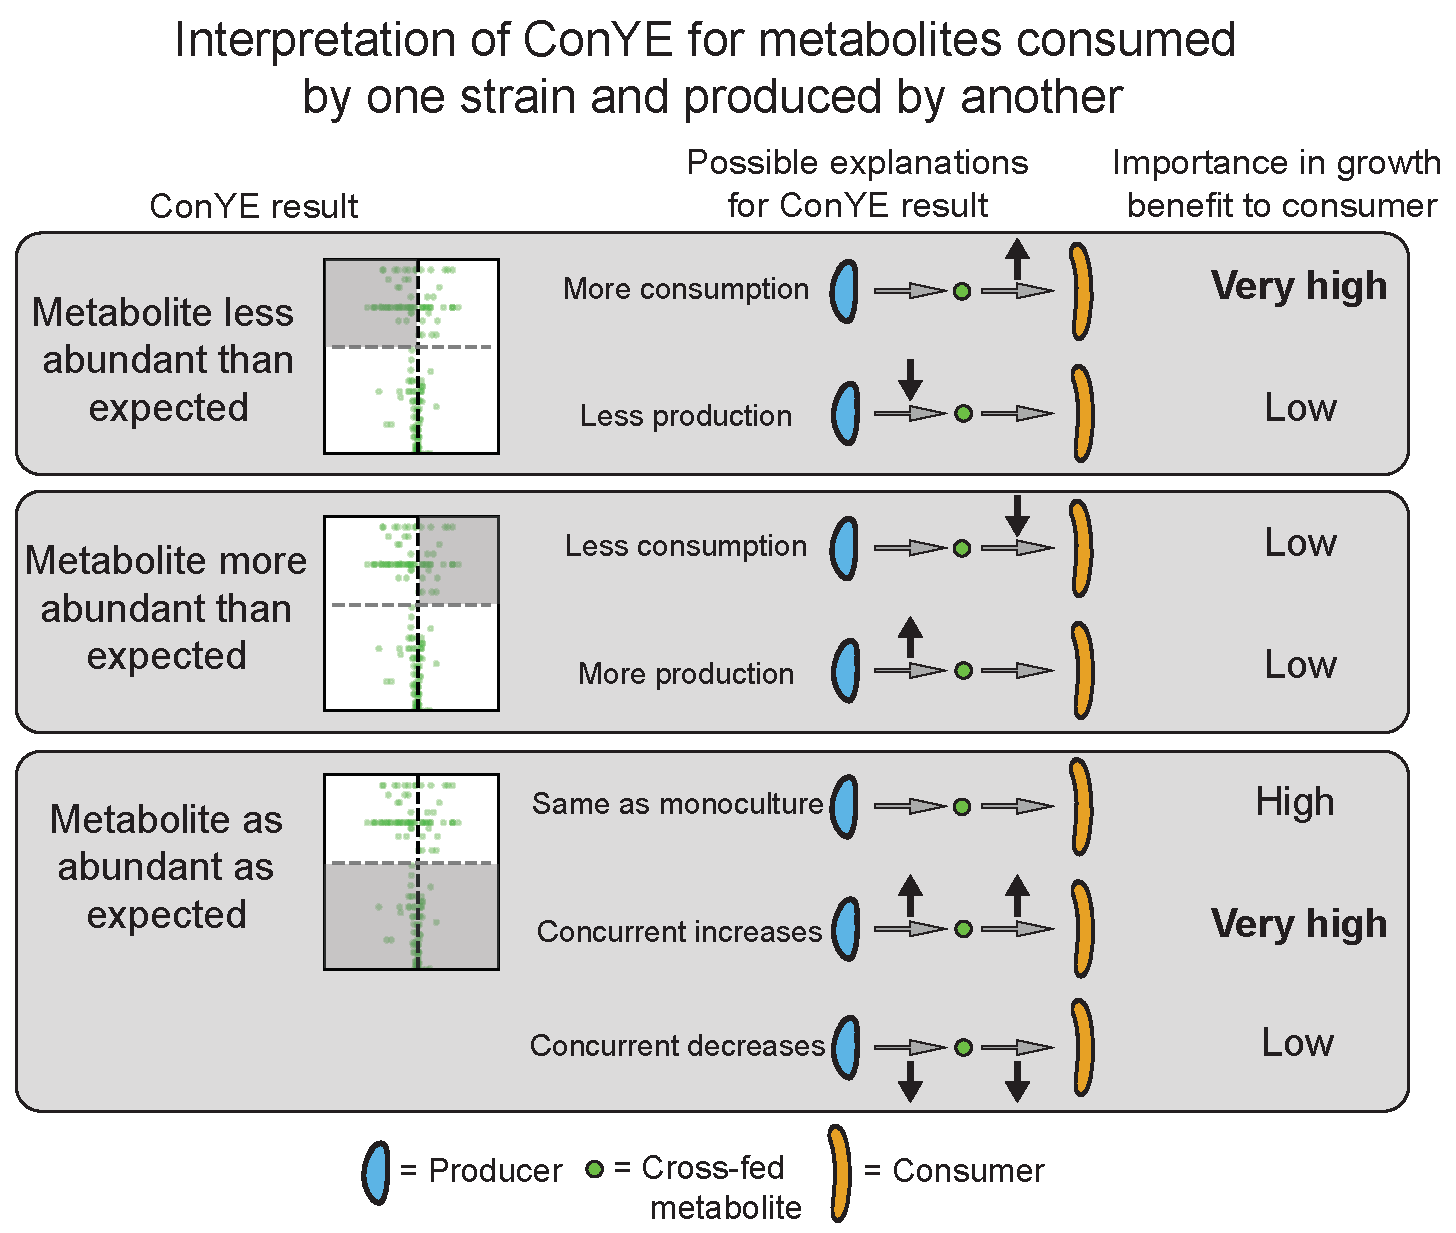
\includegraphics[width=\linewidth]{ch2_fig5}
\caption[Interpretations of ConYE results for metabolites consumed by one strain in monoculture and produced by another strain in monoculture.]{\textbf{Interpretations of ConYE results for metabolites consumed by one strain in monoculture and produced by another strain in monoculture.} In this example, the consumer experienced a growth benefit. The shaded region of each volcano plot describes the points that fall into the category described on left. In “Importance in growth benefit to consumer” column, the entry for each scenario assumes that consumption of the metabolite is coupled with biomass production. The importance assignments are qualitative, and reflect whether the consumer experienced an increase in metabolite flux in the explanatory scenario (high for increased flux, low for decreased flux).}
\end{figure}

\subsubsection{Co-culture increases the efficiency of metabolite utilization}

After applying ConYE to all co-cultures, the null hypothesis was rejected for 500/1290 metabolites (38.8\%; 86 metabolites tested across 15 co-culture conditions, resulting in 1290 comparisons), suggesting that co-culture alters metabolism of a substantial portion of metabolites when taking into account changes in growth during co-culture. For metabolites that were consumed by one or both strains in monoculture, the amount consumed per unit of strain growth generally decreased in co-culture if the null hypothesis was rejected. Specifically, of the 624 instances of metabolites that fell into this category, 151 (24.2\%) were significantly more abundant than expected in co-culture, whereas 94 (15.1\%) were less abundant than expected (Figure 2.4C, left). Of the 278 instances of a metabolite being produced by one or both strains in a pairing in monoculture, 71 (25.5\%) were less abundant than expected, while 27 (9.7\%) were more abundant than expected (Figure 2.4C, middle). Thus, although co-culture often resulted in a greater quantity of a metabolite being produced relative to either monoculture (i.e. metabolites driving monoculture and co-culture separation in PCA, Figure 2.3B), the amount produced relative to growth of each strain decreased for most metabolites. Similarly, the amount of each metabolite consumed relative to biomass in co-culture generally decreased. These results suggest that these co-cultures can increase the efficiency of biomass production through niche expansion (e.g. consuming metabolites they did not consume in monoculture) or cross-feeding rather than increasing consumption of metabolites they did not fully deplete in monoculture. Indeed, 90/1290 (6.98\%) metabolites were not consumed or produced by either strain in monoculture, yet were consumed when the two strains were in co-culture.

These distinct ConYE trends are enriched in cases with positive growth interactions (Figure 2.6A). When considering only pairings with a positive growth effect for at least one strain, there were 219 metabolites that were consumed by one or both strains in monoculture. Of these 219 metabolites, 138 (63.0\%) were more abundant than expected, while only 6 (2.74\%) were less abundant than expected. Of the 88 metabolites produced by one or both strains in monoculture for these co-cultures, 51 (58.0\%) were less abundant than expected, and only 5 (5.68\%) were more abundant than expected. Taken together, these results indicate that co-cultures with positive interactions are able to more efficiently utilize resources than co-cultures without positive interactions or monocultures.

There are three mechanisms that may enable this phenotype: niche expansion (consumption of metabolites not consumed in monoculture), cross-feeding, and detoxification via consumption of growth-inhibiting metabolites. In co-culture, the subset of strain pairs with positive interactions consumed 30 metabolites that were not consumed by either species in monoculture. Interestingly, all 30 instances of emergent metabolite consumption were carried out by \textit{Lactobacillus} ASF361+\textit{Eubacterium} ASF492, \textit{Lactobacillus} ASF361+\textit{Pseudoflavonifractor} ASF500, and \textit{Eubacterium} ASF492+\textit{Parabacteroides} ASF519, while the remaining two pairs (\textit{Clostridium} ASF356+\textit{Parabacteroides} ASF519 and \textit{Lactobacillus} ASF361+\textit{Parabacteroides} ASF519) had 0 cases of emergent consumption (See Table S3 for all cases). Given this result, it is likely that the growth benefits that occurred for \textit{Clostridium} ASF356+\textit{Parabacteroides} ASF519 and \textit{Lactobacillus} ASF361+\textit{Parabacteroides} ASF519 are due to cross-feeding or detoxification, while the growth benefits for the other positive interaction pairs are at least in part due to niche expansion.

\begin{figure*}[tb!]
\centering
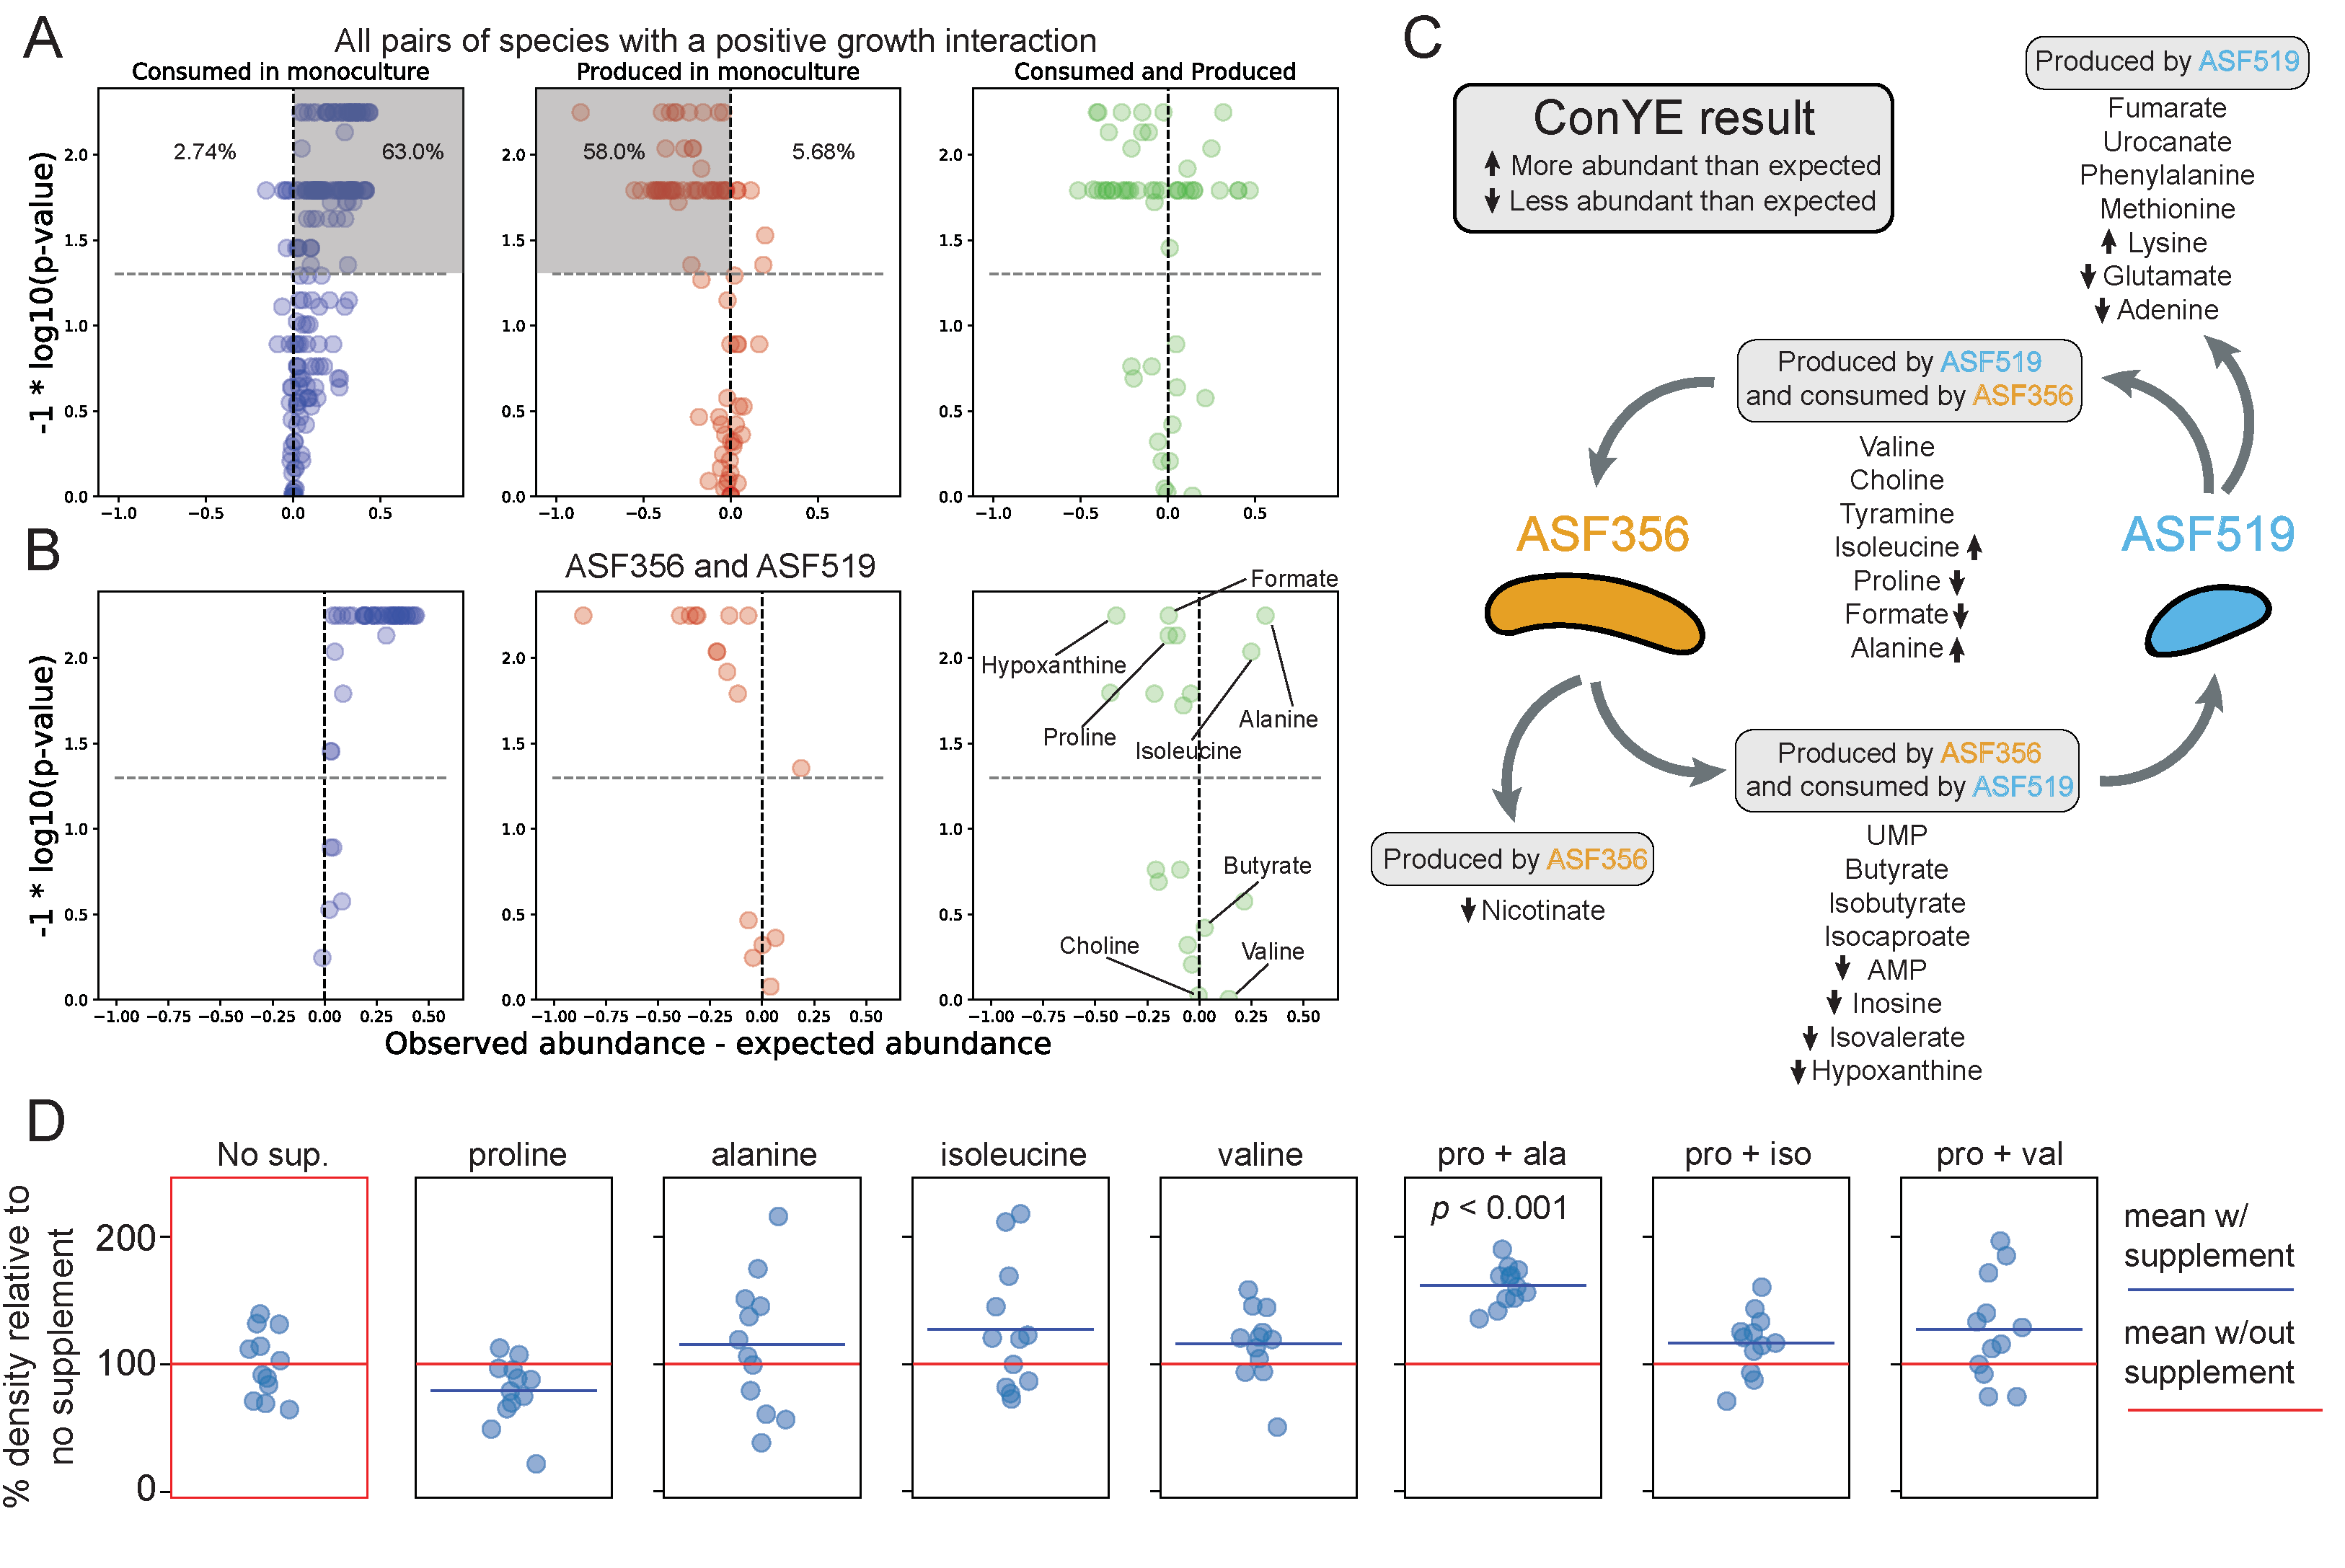
\includegraphics[width=0.9\textwidth]{ch2_fig6}
\caption[Emergent metabolism in co-culture pairings with a growth benefit and in vitro testing.]{\textbf{Emergent metabolism in co-culture pairings with a growth benefit and in vitro testing.} \textbf{A)} ConYE results for all metabolites from co-cultures with a positive growth interaction. Shaded quadrants represent consumed metabolites that were more abundant than expected (left) or less abundant than expected (middle). Percentages shown represent the number of metabolites within the plot that fall in the quadrant. \textbf{B)} ConYE results for co-culture of Clostridium ASF356 and Parabacteroides ASF519. Metabolites on right for which p > 0.05 are labeled unless they could not be assigned an identity. Metabolites for which p < 0.05 are labeled if assigned an identity and abs(x) > 0.10 for that metabolite. x and y axes are scaled as in Figure 4. \textbf{C)} Metabolic interaction topology for Clostridium ASF356 and Parabacteroides ASF519. ConYE results are indicated with arrows pointing up or down for metabolites for which the null hypothesis was rejected. Metabolite classifications are based on monoculture behavior. \textbf{D)} OD600 of Clostridium ASF356 monocultures after 72 hours of growth in supplemented media conditions. ”No sup.” had no supplement added, while conditions with a single amino acid were supplemented at 1.25g/L. In conditions with two supplements, each metabolite is supplemented at 1.25g/L. “pro + ala”, “pro + iso”, and “pro + val” conditions include L-proline with L-alanine, L-isoleucine, or L-valine, respectively.}
\end{figure*}

\subsubsection{Identifying cross-fed metabolites and evaluating feasibility \textit{in silico}}

We next sought to investigate potential cross-fed metabolites from ConYE for co-cultures with positive growth interactions in order to find a mechanism that explained, at least in part, the growth benefit. For this task, we focused on the co-culture of \textit{Clostridium} ASF356 and \textit{Parabacteroides} ASF519 to exclude co-cultures which may have engaged in niche expansion (and therefore cross-feeding may have played a more minor role in observed growth benefits) and to remove the need to consider additional confounding factors introduced by a strong negative growth interaction (e.g. negative impact on \textit{Parabacteroides} ASF519 growth in co-culture with \textit{Lactobacillus ASF361}). Seven named metabolites were consumed by \textit{Clostridium} ASF356 in monoculture that were also produced by \textit{Parabacteroides} ASF519 in monoculture (Figure 2.6B; labelled metabolites satisfy criteria specified in figure caption). Of those 7 metabolites, tyramine, valine, and choline did not result in rejecting the ConYE null hypothesis. Isoleucine and alanine were more abundant than expected, and proline and formate were less abundant than expected. Isoleucine and alanine may have been cross-fed, but given that they were more abundant than expected, consumption of these metabolites only contributed to enhanced growth if \textit{Parabacteroides} ASF519 also produced less of these metabolites than expected (as in middle panel of Figure 2.5, where \textit{Parabacteroides} ASF519 is the producer and \textit{Clostridium} ASF356 is the consumer). Proline and formate were both less abundant than expected, so were either consumed by \textit{Clostridium} ASF356 more in co-culture than in monoculture (and thereby cross-fed) or produced less by \textit{Parabacteroides} ASF519 in co-culture than in monoculture (as in top panel of Figure 2.5).

ConYE can identify metabolites that are potentially cross-fed, but the actual behavior of each strain in co-culture with respect to that metabolite is difficult to infer using existing experimental techniques. Because we can only evaluate the co-culture behavior based on an expectation derived from monoculture behavior, it is still possible that co-culture leads to reduced production and consumption of those metabolites rather than cross-feeding. We sought to provide orthogonal evidence for ConYE results by evaluating the potential for metabolites to increase the growth rate of a strain in monoculture, reasoning that ConYE may produce false-positive inferences if metabolites are not actually coupled with biomass production. We chose to support inferences made using ConYE by building and applying Genome-scale metabolic network reconstructions (GENREs). GENREs are mathematical representations of all metabolic reactions that an organism can carry out, and have been used extensively to predict the effect of environmental conditions on growth of bacterial species \cite{Oberhardt2009-iu}. We created an ensemble of 100 GENREs for each strain in this study to gain greater confidence in cross-feeding predictions and to enable predictive modeling of metabolism in future studies (Figure S3A and S3B; see Methods). For each metabolite, we evaluated its impact on growth of individual strains by performing ensemble flux balance analysis (EnsembleFBA \cite{Biggs2017-md} to predict the growth rate of the strain without the metabolite available and with the metabolite available in excess (see Methods). We performed this procedure for the cross-feeding candidate metabolites between \textit{Clostridium} ASF356 and \textit{Parabacteroides} ASF519. If a metabolite increases the predicted \textit{in silico} growth rate when available in excess, we take that as parallel evidence to support or oppose the ConYE-based inferences. EnsembleFBA results are summarized in Figure S3 for all metabolites except tyramine, which was not present in any GENREs within the ensemble for \textit{Clostridium} ASF356.

\begin{figure*}[tb]
\centering
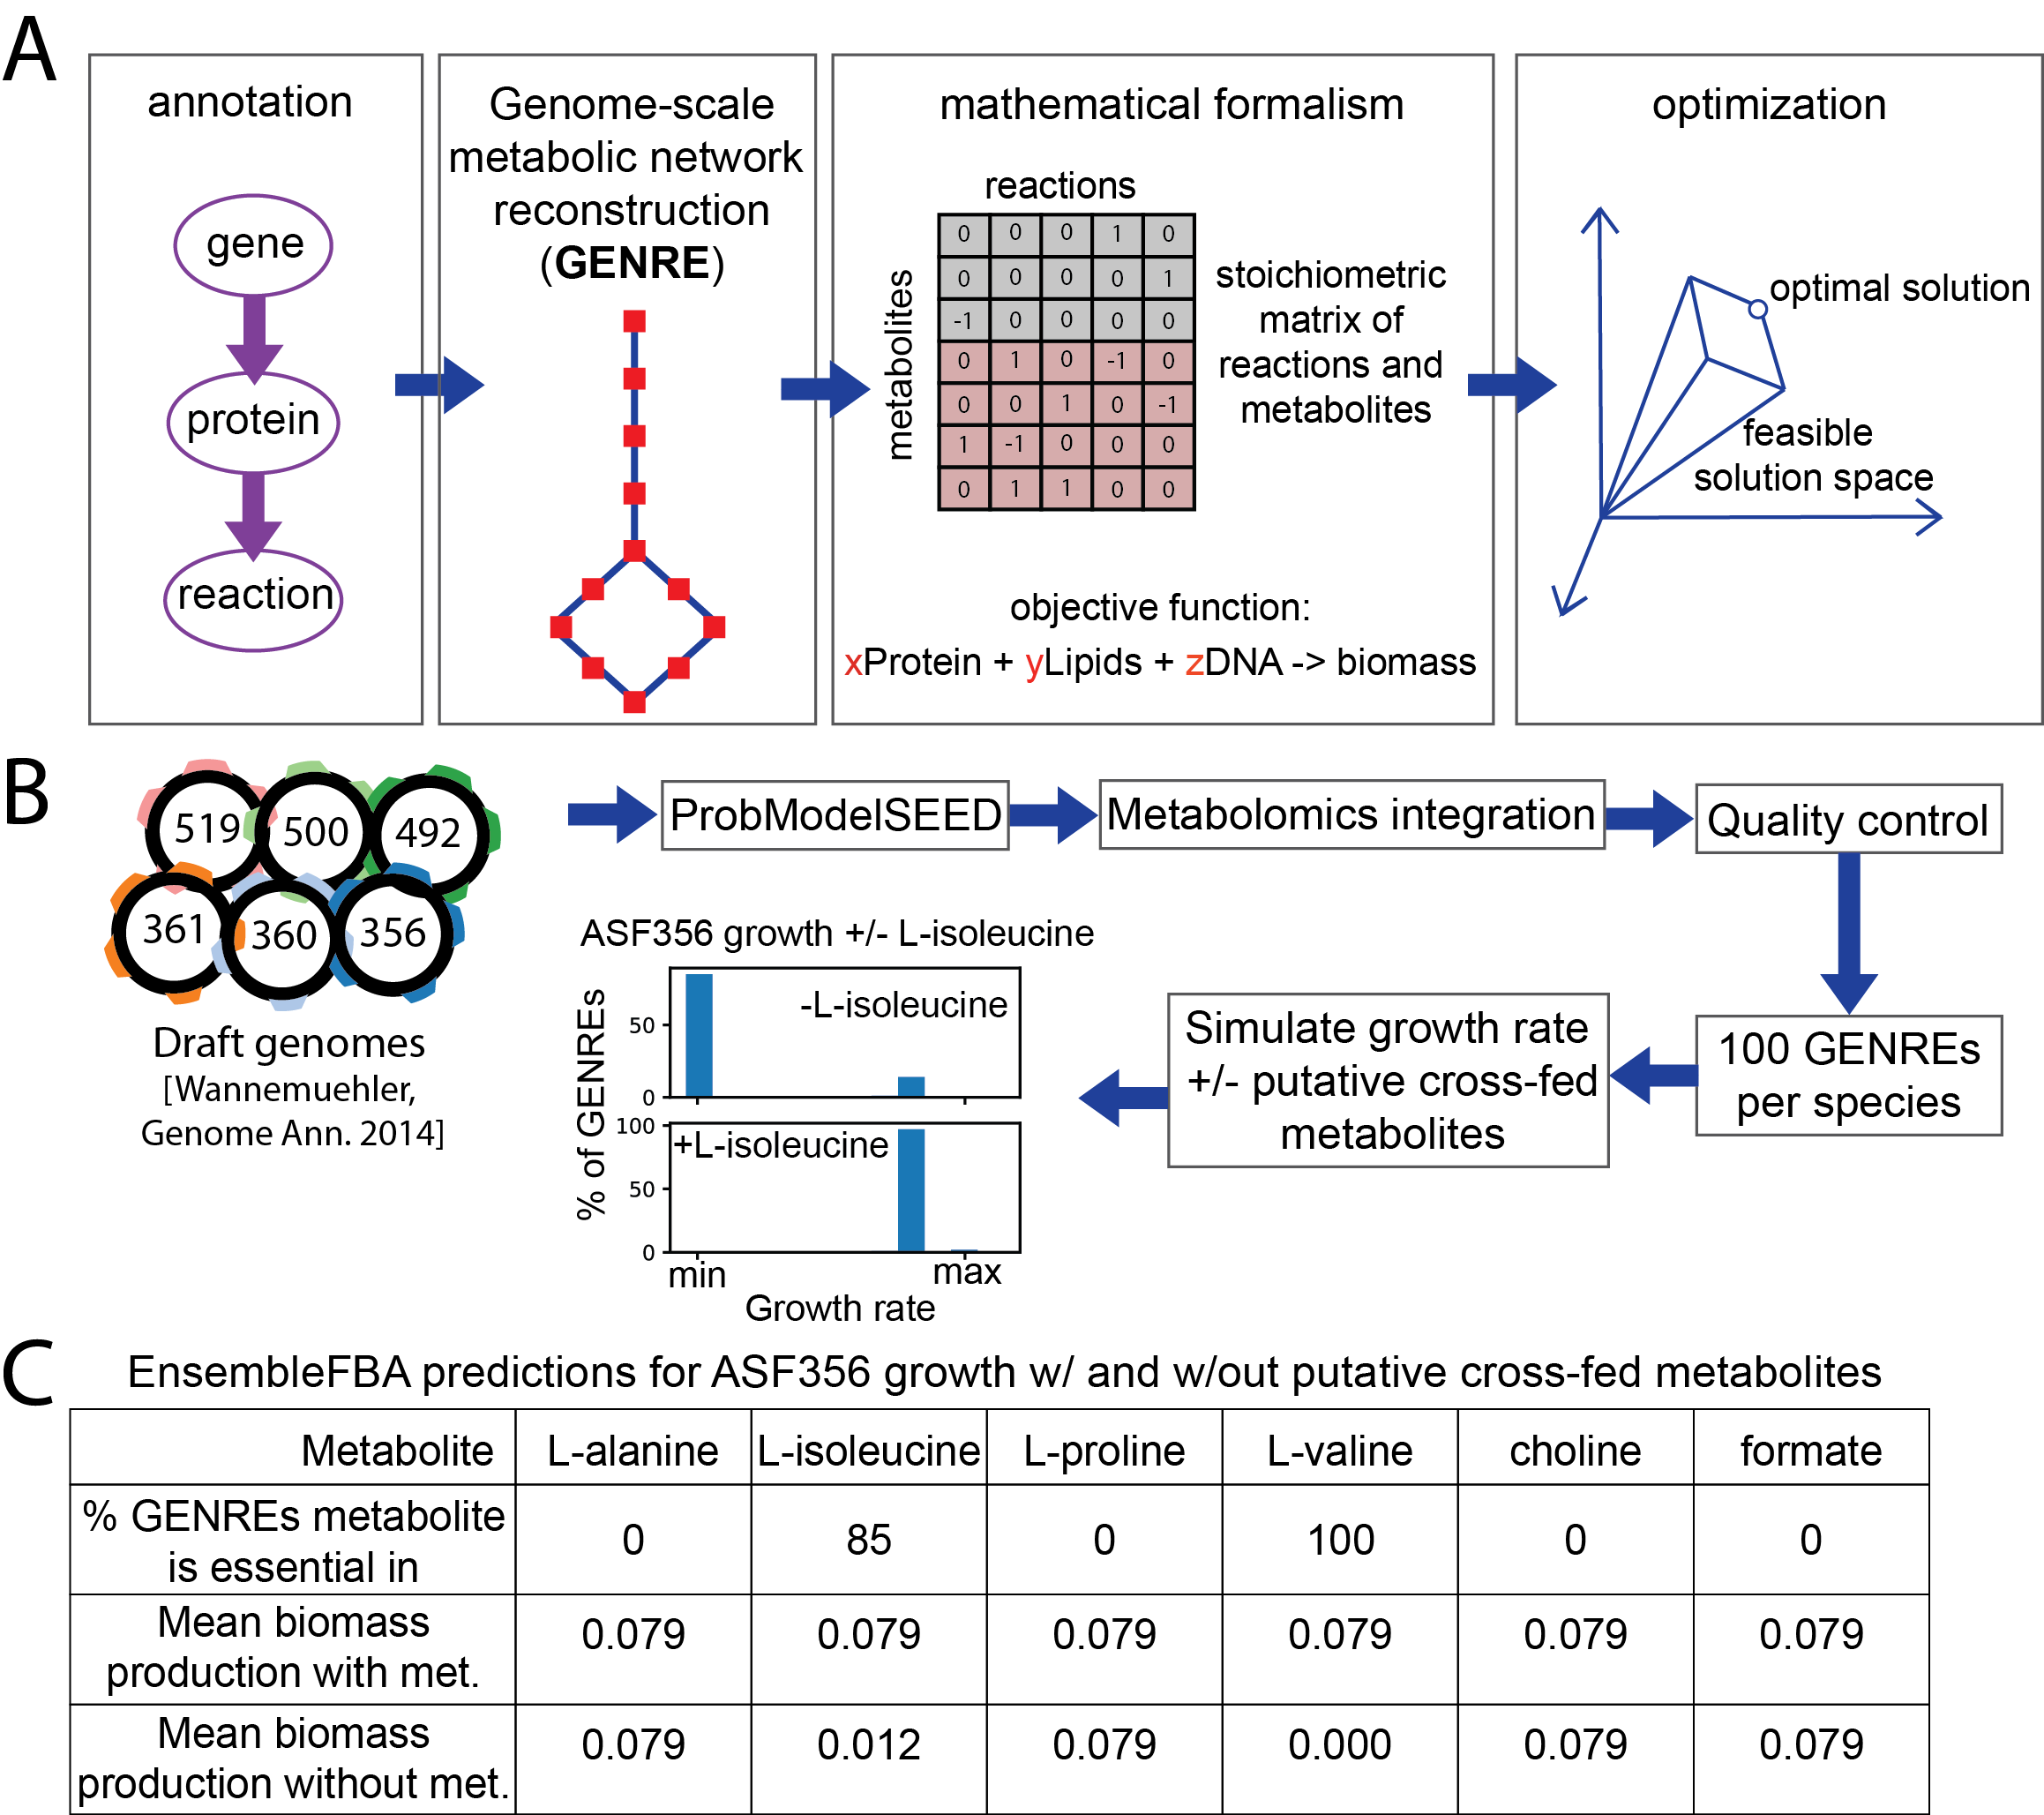
\includegraphics[width=0.8\textwidth]{ch2_figS3}
\caption[Computational model-driven interrogation of potential metabolic interactions and experimental validation of a cross-feeding interaction.]{\textbf{Computational model-driven interrogation of potential metabolic interactions}  \textbf{A)} Process for generating and applying a genome-scale metabolic network reconstruction (GENRE). \textbf{B)} Novel pipeline for constructing and analyzing ensembles of GENREs for the ASF strains. Details for each step in Methods. \textbf{C)} EnsembleFBA predictions of the influence of potentially cross-fed metabolites on growth of \textit{Clostridium} ASF356. Biomass production values are for flux through the biomass reaction in units of hour-1, and a metabolite was considered essential if removal led to flux through the biomass reaction of less than < 1E-5/hour. Predicted flux through biomass in the experimental medium without any supplement or metabolite removal is 0.079/hour.}
\end{figure*}

Valine was essential for growth of \textit{Clostridium ASF356} in all 100 GENREs in its ensemble. Isoleucine was essential for 85/100 GENREs but had no effect on growth for the other 15 GENREs, while absence of the rest of the potentially cross-fed metabolites had no effect on predicted growth rate. Given the \textit{in silico} essentiality of valine and the ConYE results indicating valine was as abundant as expected, valine may have conferred a growth benefit to \textit{Clostridium} ASF356 if cross-fed between \textit{Clostridium} ASF356 and \textit{Parabacteroides} ASF519. While isoleucine was essential for growth of the majority of GENREs in the \textit{Clostridium} ASF356 ensemble, there was a subset of GENREs in which its removal had no effect. Given this \textit{in silico} uncertainty, as well as the ConYE result which indicated it was more abundant than expected in co-culture, we hypothesized that cross-feeding of isoleucine may not have influenced growth of \textit{Clostridium} ASF356 as much as valine. Alanine, proline, choline, and formate were not essential and did not influence predicted growth rates \textit{in silico}. Critically, however, this analysis indicated that availability of any of the individual metabolites in excess did not confer a growth benefit relative to the unsupplemented medium.

\subsubsection{\textit{In vitro} investigation of an inferred cross-feeding interaction}

Given the lack of an \textit{in silico} prediction which indicated that supplementation of a putatively-crossfed metabolite would increase the growth rate of \textit{Clostridium} ASF356, we considered mechanisms through which the metabolites discussed above may interact with each other to influence growth, rather than in isolation as considered thus far. \textit{Clostridium} ASF356 belongs to the \textit{Clostridium} genus, throughout which amino acid fermentation via Stickland reactions is common \cite{Mead1971-oa}. Stickland reactions involve coupling the oxidative deamination of one amino acid with the reductive decarboxylation of another amino acid, producing two short-chain fatty acids or branched chain fatty acids that each contain one fewer carbon than the respective amino acid from which they were derived \cite{Nisman1954-xl}. Proline, glycine, hydroxyproline, and ornithine are strong Stickland reaction electron acceptors, while alanine, valine, leucine, and isoleucine are strong electron donors. We observed that \textit{Clostridium} ASF356 consumed proline, a strong electron acceptor, and all the listed electron donors in monoculture, while \textit{Parabacteroides} ASF519 produced proline, alanine, valine, and isoleucine and consumed leucine in monoculture. In co-culture, ConYE indicated that proline was significantly less abundant than expected, suggesting it was consumed more per unit biomass in co-culture than in monoculture. Given this observation and the lack of growth rate increase predicted \textit{in silico} with excess proline available, we hypothesized that proline was of critical importance to the growth benefit for \textit{Clostridium ASF356} in co-culture with \textit{Parabacteroides} ASF519, but depended on the presence of suitable electron donors. Behavior varied amongst the electron donors that may pair with proline in the Stickland reaction: isoleucine and alanine were more abundant than expected, while valine was as abundant as expected. The Stickland fermentation product for proline is 5-aminovalerate, which we could not identify within the NMR spectra due to spectral overlap with other metabolites and lack of signal in regions unique to 5-aminovalerate. The products for isoleucine, valine, and alanine are valeric acid (not detected), isobutyrate (as abundant as expected), and acetate (less abundant than expected), respectively. Decreased abundance of leucine, which is fermented to isovalerate (less abundant than expected), in co-culture suggests decreased consumption by \textit{Clostridium} ASF356 or increased consumption of isovalerate by \textit{Parabacteroides} ASF519, which consumed isovalerate in monoculture.

To test the hypothesis that \textit{Clostridium} ASF356 experiences a growth benefit in the presence of proline and suitable electron donors, we grew \textit{Clostridium} ASF356 in media supplemented with proline, alanine, isoleucine, valine, or each combination of the three electron donors (alanine, isoleucine, valine) with proline. NMR spectroscopy cannot differentiate between amino acid isomers, so we assumed all amino acids consumed and produced were the L- isoform (as in tryptone, the major source of amino acids in the medium). Organisms conducting Stickland fermentation of proline generally possess a proline racemase, since D-proline is the isoform that is fermented \cite{Watanabe2015-wa}. Leucine was consumed by both strains in monoculture, thus was excluded because it was unlikely to be cross-fed in co-culture. Only the monoculture supplemented with both proline and alanine had increased density relative to no supplement (Figure 2.6D, \textit{p} < 0.05, Mann-Whitney U-test with false discovery rate control using Benjamini-Hochberg procedure), suggesting that co-metabolism of proline and alanine contributes to growth of \textit{Clostridium} ASF356. Given that the ConYE results indicated that alanine was more abundant in co-culture than expected, the results of the supplementation experiment imply that production of alanine by \textit{Parabacteroides} ASF519 was increased in co-culture with \textit{Clostridium} ASF356 or that \textit{Clostridium} ASF356 used alanine more efficiently in co-culture. Additionally, the lack of growth benefit conferred by supplementation of proline with isoleucine or valine suggests that any change attributable to pairing either electron donor with proline was too small to detect given our sample size. Formate can also be used as an electron donor for proline reduction in the Stickland reaction \cite{Kabisch1999-jf}, which we did not factor into our experiments. Formate was produced by \textit{Parabacteroides} ASF519 and consumed by \textit{Clostridium} ASF356 in monoculture, and was less abundant than expected in co-culture according to ConYE. Thus, formate may have also contributed to the observed growth benefit.

After performing these supplementation experiments, we attempted identification of 5-aminovalerate in the supernatant from \textit{Clostridium} ASF356 and \textit{Parabacteroides} ASF519 co-culture using 2D $^1\!$H homonuclear correlation spectroscopy (COSY), which can identify metabolites with overlap in 1D NMR spectra (Figure S5; Methods). 5-aminovalerate was not present at detectable quantities; the peaks within the overlapping region which we suspected to contain 5-aminovalerate were from valine and gamma-aminobutyrate (GABA). Thus, Stickland fermentation only occurred if 5-aminovalerate was further degraded. Such activity has been observed in \textit{Clostridium viride} (formerly \textit{Clostridium aminovalericum}), which converts 5-aminovalerate to valerate, acetate, propionate, and ammonia \cite{Barker1985-rs,Barker1987-jt}. Additionally, synthesis of GABA from glutamate is broadly distributed in plants and bacteria, and the responsible enzyme in some organisms is known to convert 5-aminovalerate to glutamate via promiscuous 5-aminovalerate transaminase activity \cite{Shin2016-vy,Yonaha1985-xp}. Both \textit{Clostridium} ASF356 and \textit{Parabacteroides} ASF519 have multiple putative proteins similar to known 5-aminovalerate transaminase enzymes (BLAST E value < 1E-50, 31-34\% identity; compared to gabT gene from \textit{Pseudomonas putida} KT2440), so either strain may be capable of producing GABA from 5-aminovalerate.

\begin{figure*}[tb]
\centering
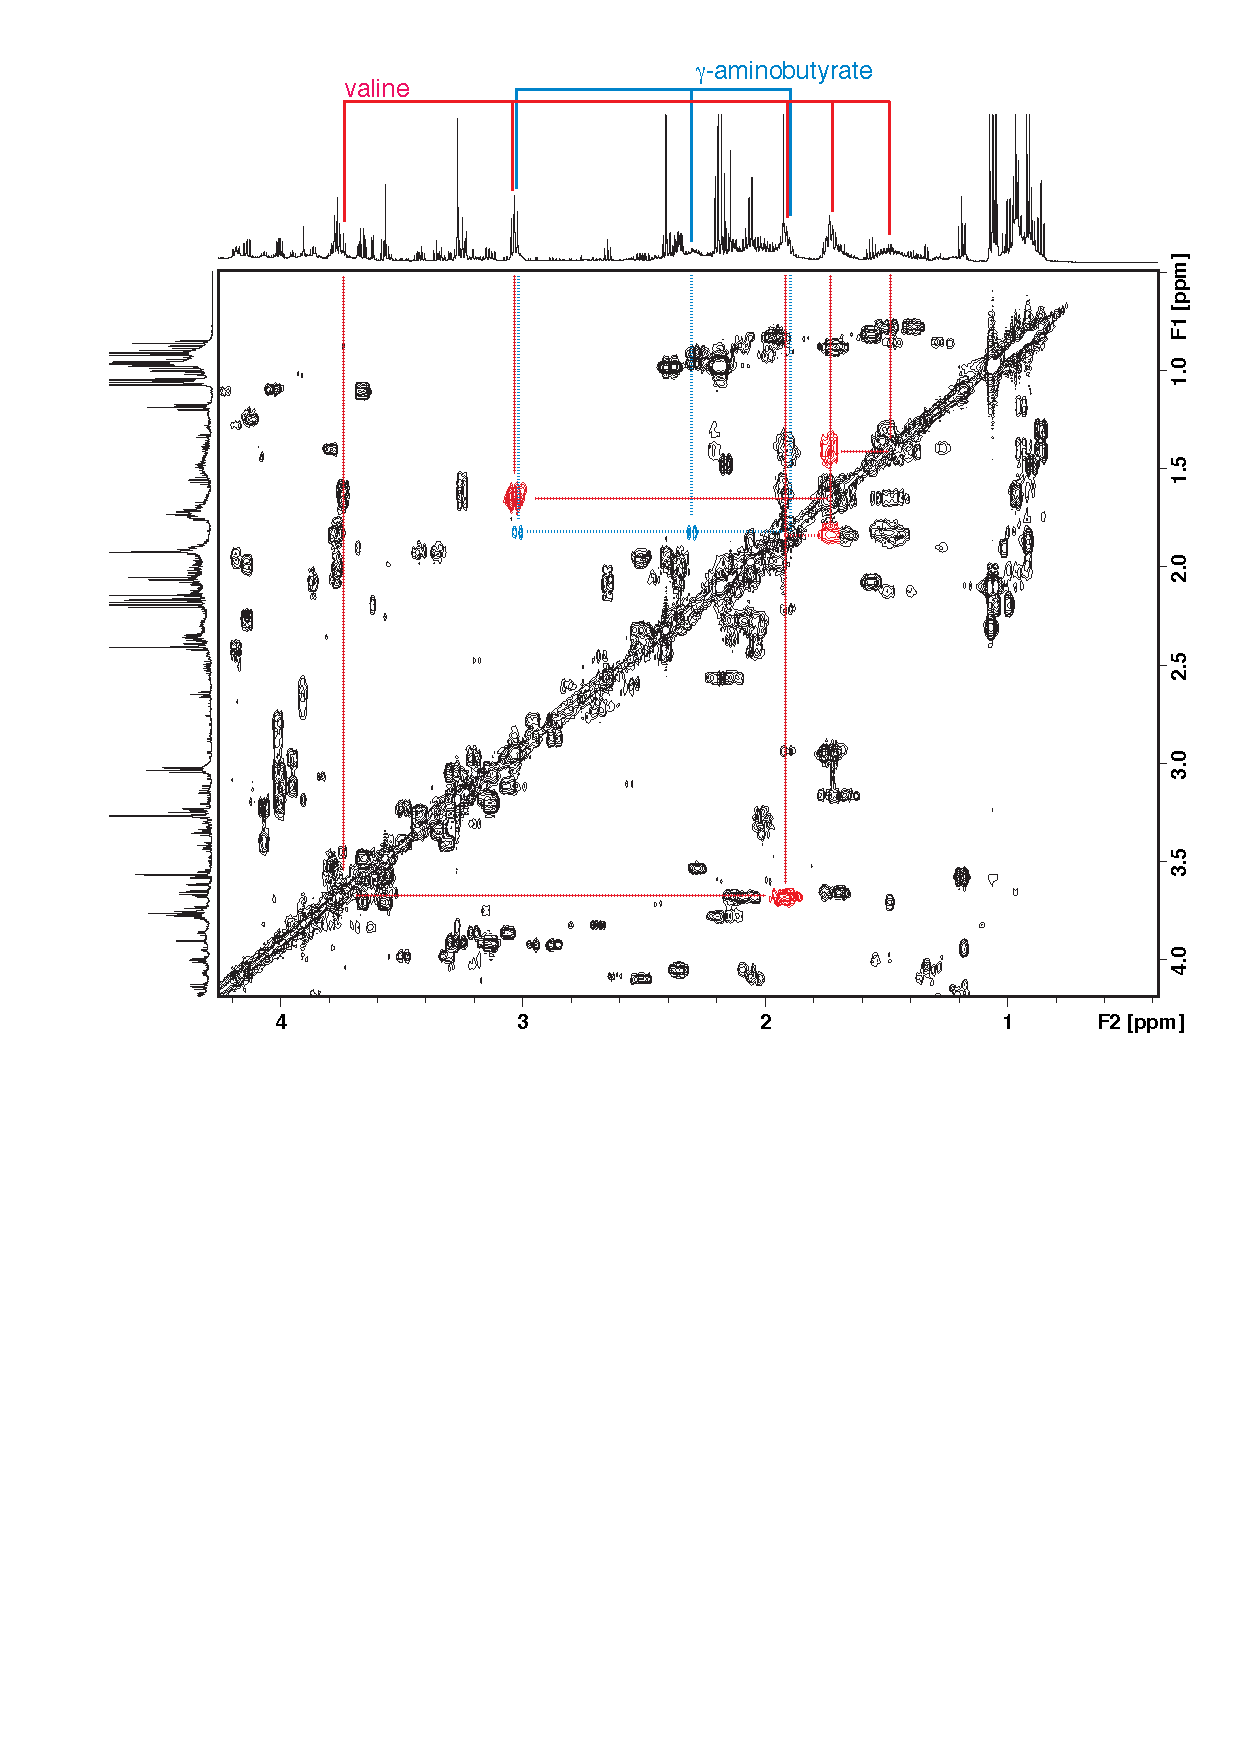
\includegraphics[width=0.8\textwidth]{ch2_figS5}
\caption[2D $^1\!$H NMR spectra collected on a single sample of supernatant from co-culture of \textit{Clostridium} ASF356 and \textit{Parabacteroides} ASF519]{\textbf{2D $^1\!$H NMR spectra collected on a single sample of supernatant from co-culture of \textit{Clostridium} ASF356 and \textit{Parabacteroides} ASF519} 2D spectra show gamma-aminobutyrate, not 5-aminovalerate, in the region overlapping with valine in 1D. Peaks corresponding to valine shown in red, gamma-aminobutyrate shown in blue.}
\end{figure*}

We also tested the effect of concurrent supplementation with Stickland pairs \textit{in silico}, which did not lead to any predicted growth benefit because the GENREs do not contain Stickland fermentation reactions. Stickland reactions are absent from reaction databases used to construct and curate GENREs such as the ModelSEED biochemistry database \cite{Henry2010-um}, but are present in the AGORA resource of semi-automatically generated GENREs for gut microbes \cite{Magnusdottir2017-dk}. None of the genes involved in Stickland fermentation have been identified in the genome of \textit{Clostridium} ASF356 as of this writing (determined via searching the annotated \textit{Clostridium} ASF356 genome in PATRIC \cite{Wattam2017-tk}, BLAST against D-proline reductase gene subunits). Taken together, these results suggest that proline and alanine co-supplementation confers a growth benefit through an alternative pathway or through Stickland fermentation with subsequent breakdown of 5-aminovalerate.


\section{Discussion}

In this study, we used data-driven methods to identify metabolic signatures that may contribute growth modulation in bacterial co-cultures, proposed mechanisms by which a specific signature may arise, and verified that growth of the benefiting strain is enhanced when putatively-crossfed metabolites are supplemented \textit{in vitro}. The biochemical capability we evaluated experimentally, Stickland fermentation of proline and alanine, is widely distributed in proteolytic \textit{Clostridia} \cite{Mead1971-oa}. While the ability of species inhabiting the mammalian gut to perform Stickland fermentation has been investigated, this study connects possible Stickland fermentation to a metabolic interspecies interaction that modulates growth. Given that some of the end products of Stickland fermentation were present at low concentrations in the fresh medium, and that \textit{Parabacteroides} ASF519 consumed them in monoculture (isobutyrate, isovalerate, and isocaproate), our data suggest that this interaction may be bidirectional. This observation supports some theoretical motifs for metabolism in the gastrointestinal tract proposed in the literature, such as the model of carbon and nitrogen flow proposed by Fischbach and Sonnenburg in which \textit{Clostridia} (e.g. \textit{Clostridium} ASF356) ferment amino acids, providing ammonium and other amino acid fermentation products to \textit{Bacteroides} (e.g. \textit{Parabacteroides} ASF519, which was assigned to the genus Bacteroides prior to 2006) \cite{Fischbach2011-wg,Sakamoto2006-oz}. \textit{Clostridium} ASF356 and \textit{Parabacteroides} ASF519 are co-located along the mouse gastrointestinal tract, however the relevance of this observation is unclear given a microbiota as restricted in size as the ASF \cite{Sarma-Rupavtarm2004-jv}. This kind of interaction has direct relevance to enteric pathogens, as emerging evidence indicates that in vivo utilization of proline via Stickland fermentation is highly active in \textit{Clostridium difficile} during sustained infection in mice \cite{Fletcher2018-ws,Jenior2017-lv,Jenior2017-zv}.

We expect that the growth outcome observed in the co-culture of \textit{Clostridium} ASF356 and \textit{Parabacteroides} ASF519 is due to a multitude of interactions that each have a small effect. An alternative mechanism by which co-culture could enhance growth is consumption of growth-inhibiting metabolite products. Although we did not explore them in this study, ConYE identified several cases in which this process may have occurred. For example, in the co-culture of \textit{Lactobacillus} ASF361 and \textit{Parabacteroides} ASF519, lactate, hypoxanthine, AMP, and UMP were all metabolites produced by \textit{Lactobacillus} ASF361 and consumed by \textit{Parabacteroides} ASF519 that were less abundant than expected in co-culture. Of these metabolites, lactate is known to have potent antimicrobial properties both broadly and against \textit{Lactobacillus spp.}\cite{Shelef1994-lb}, thus it is a reasonable candidate for this mechanism.

We developed ConYE to interrogate growth-modulating interactions within this study, but the framework can be used to study interspecies interactions that alter other phenotypes of interest. For example, the same analyses conducted here could be performed using consumption of a substrate of interest, such as lactose, to calculate metabolite yields as a function of that substrate rather than as a function of strain abundance. In this scenario, ConYE could be used to identify co-culture pairings that enhance conversion of lactose to a metabolite of interest, and identify cross-fed metabolites that contribute to enhanced yield of that metabolite of interest.

There is increasing interest in developing methods for inference of growth or abundance-modulating interactions between microbes from various data types and environments \cite{Friedman2017-zn,Weiss2016-tq,Xiao2017-yl}. These methods have primarily been focused on discovering interspecies interactions and the role they might play in ecosystem function, rather than ascribing mechanism to those interactions. Interspecies interactions are likely to be highly context-dependent, so more detailed knowledge about mechanisms of interaction is necessary to generalize these findings \cite{Chamberlain2014-nt}. Several approaches that integrate the metabolic and/or spatial environment using genome-scale metabolic models have been developed that account for context dependency \cite{Chan2017-tk,Harcombe2014-ev,Zomorrodi2012-ja}. However, limitations in biochemical knowledge across the bacterial tree of life limit their broad application to other organisms. Large-scale efforts to collect and assimilate biochemical knowledge of gut microbes within genome-scale metabolic models are in progress, but experimental data to validate and improve the predictive ability of these models is lacking \cite{Magnusdottir2017-dk}. Recent work to determine defined growth conditions for gut microbes will accelerate the process of experimental validation for such models, but data are still extremely sparse relative to organisms for which highly predictive metabolic models have been developed \cite{Tramontano2018-xz}. Similar metabolic model-based approaches have been applied to simplified versions of communities such as the human gut microbiota \cite{Bauer2017-kf,Chan2017-tk}, but the poor experimental tractability of these systems makes testing predicted interspecies interactions challenging and thus they are left unvalidated.

Incorporating dynamic substrate utilization information may be able to provide more accurate insight into metabolic interactions than the method we present. We envision that our method may be used as an efficient screening step in which many species are grown across many media conditions to identify putative interactions. Then, in conditions with many putative interactions, sampling can be performed with finer time resolution to attain a clearer picture of the actual coupling of metabolite consumption and production with changes in growth of individual species, as previously performed with yeast and lactic-acid bacteria \cite{Ponomarova2017-ob}. This framework, and others that model substrate utilization within a microbial community over time, could be modified with the strain abundance normalization procedure used within ConYE to identify dynamic features of emergent metabolic behavior in these communities \cite{Erbilgin2017-la}.

We have developed an experimental and computational pipeline to probe interspecies interactions and infer putative metabolic mechanisms of interaction, generating testable hypotheses.  Understanding mechanisms of interspecies interaction and the environmental conditions that induce them is a prerequisite to engineering communities with specific therapeutic or industrial value. For generalizable methods that predict interspecies interaction using mechanistic models to be successful, methods must be validated experimentally. This task will require a substantially larger set of observed interspecies interactions than are presented here, or are available in the literature, from which to derive generalizable principles. Extending our approach and similar methods to defined communities across conditions that are more diverse, both in terms of resource availability and spatial structure, will begin to make predictive modeling of interspecies interactions tractable.

\section{Conclusion}

new conclusion section

\section{Methods}
\subsubsection{A methods subsection}
This is in the subsection

\section{Acknowledgments}

Acknowledgements


\section{References}
\printbibliography[heading=none]

\section{Supplemental Figures}

\begin{figure*}
\centering
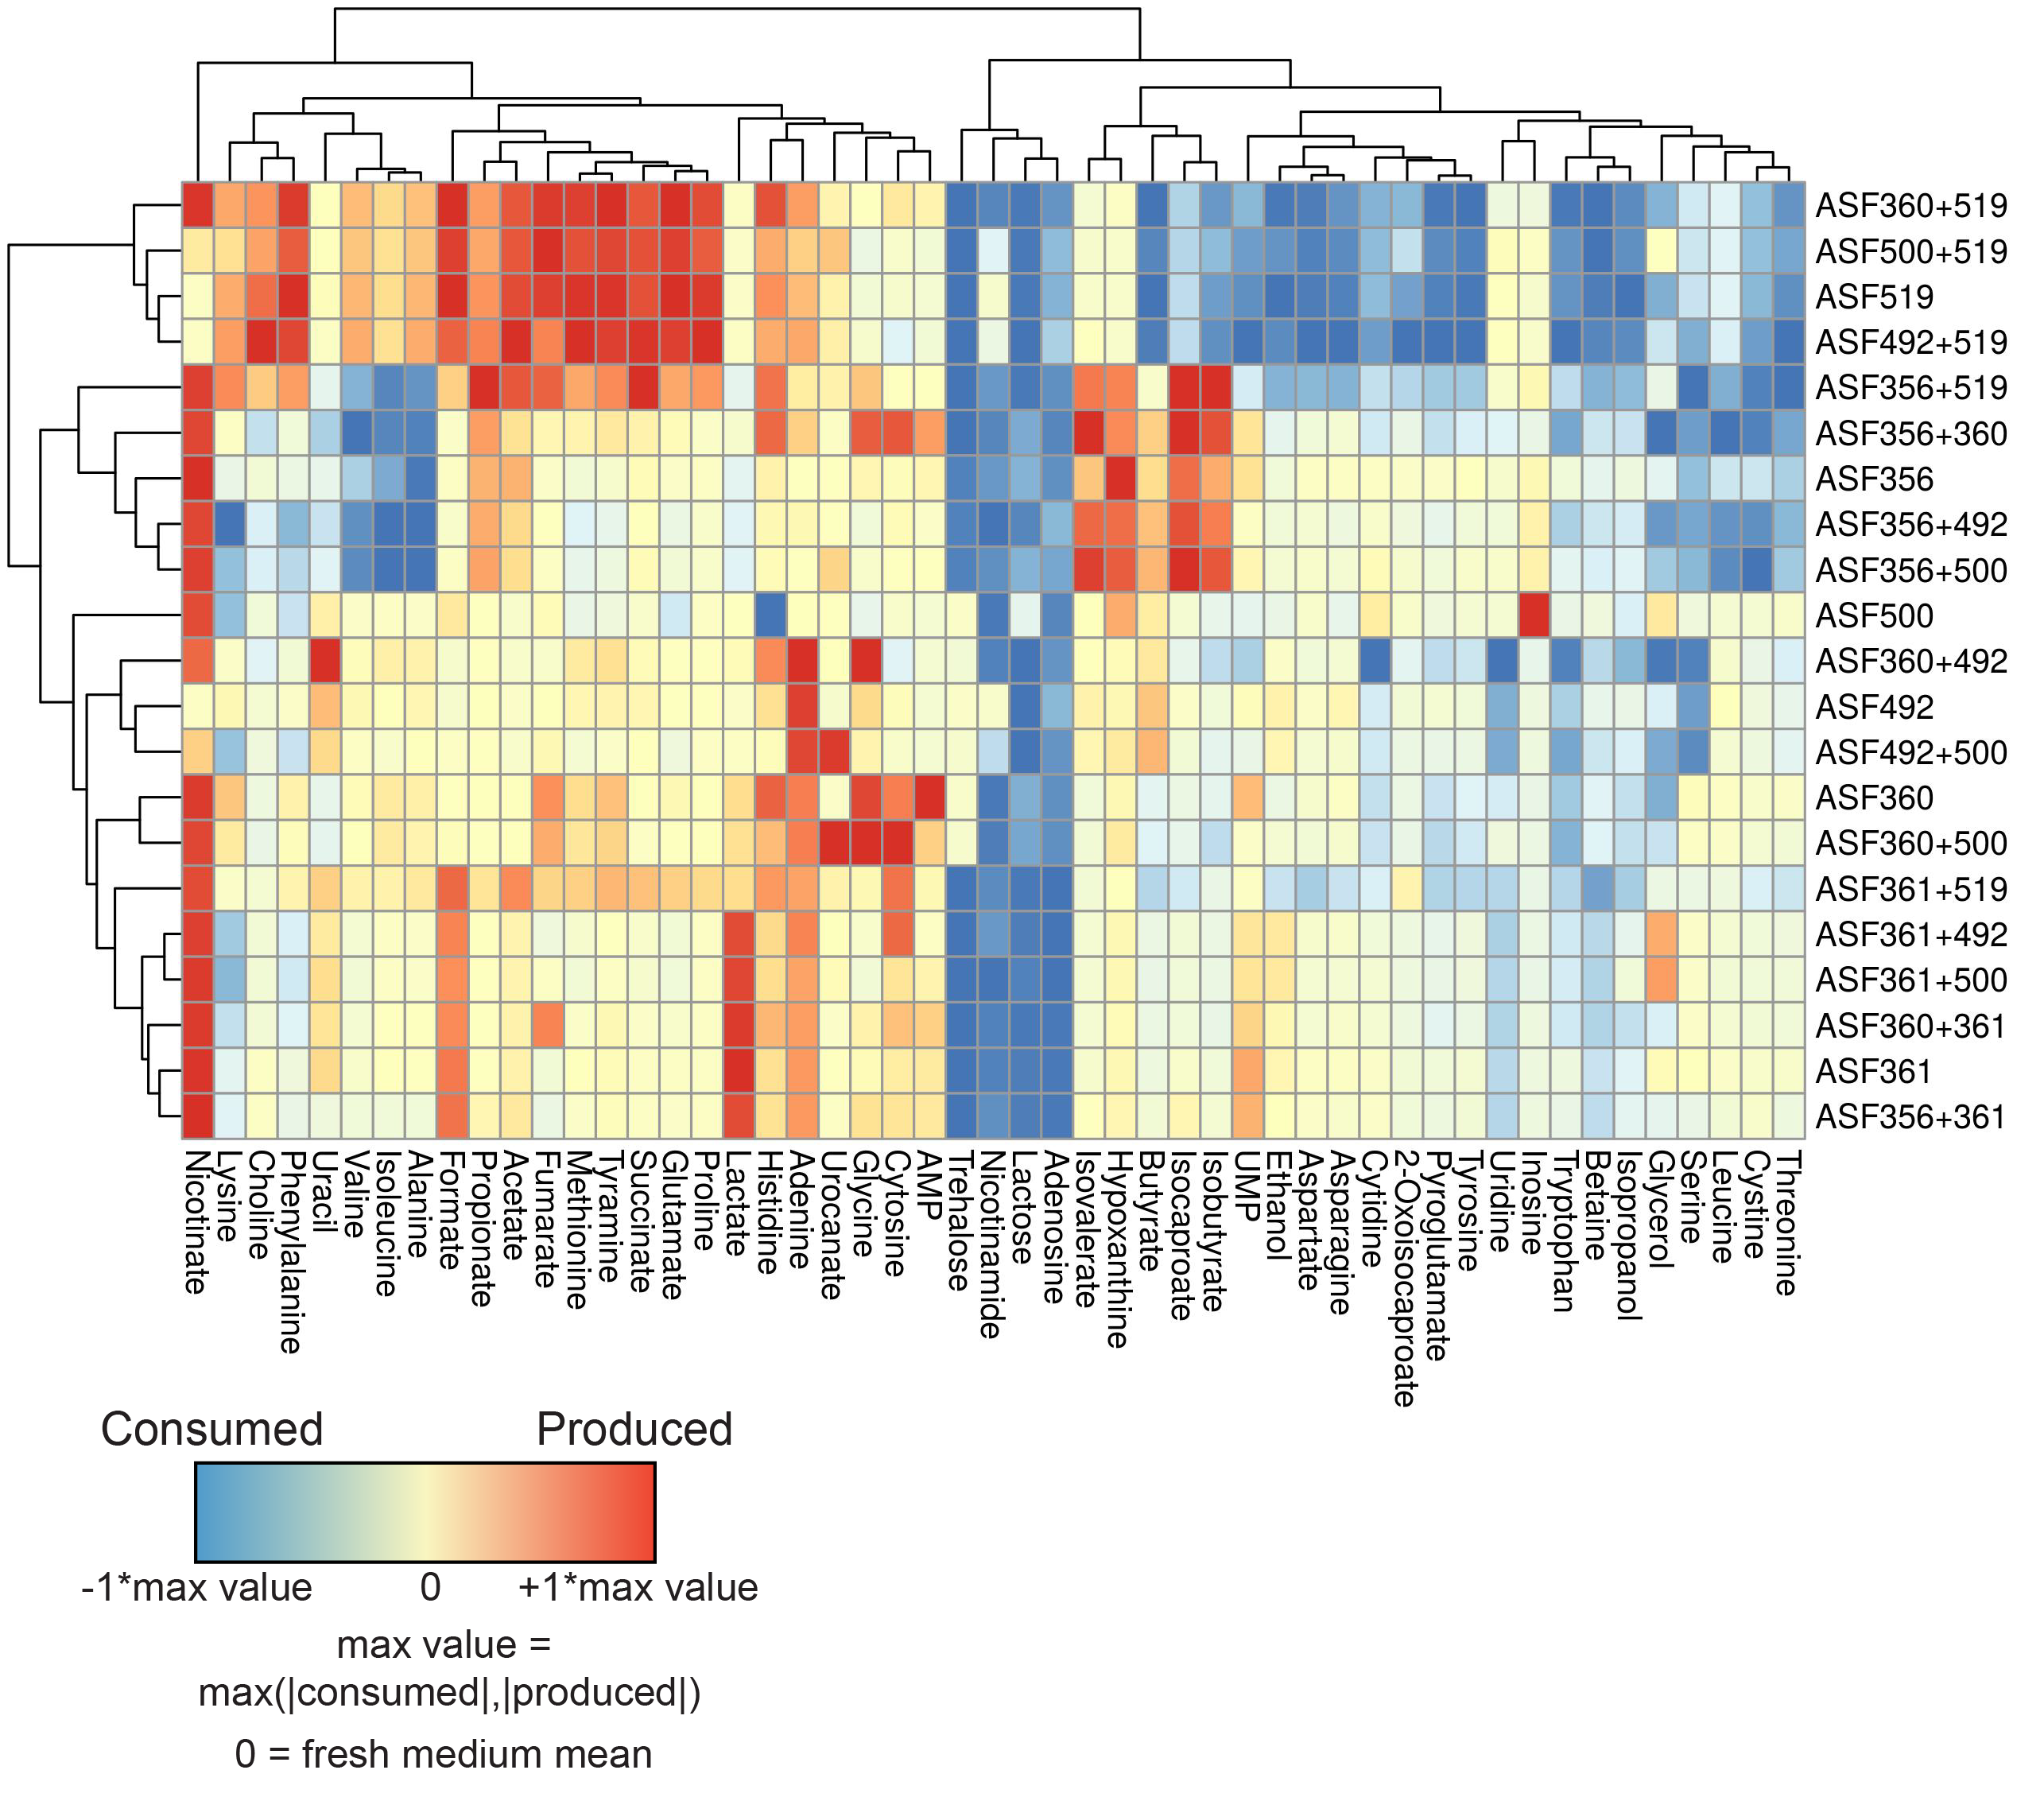
\includegraphics[width=0.8\textwidth]{ch2_figS1}
\caption[Heatmap describing supernatant metabolomes for all mono- and co-cultures after growth.]{\textbf{Heatmap describing supernatant metabolomes for all mono- and co-cultures after growth.} Red indicates higher concentration than fresh medium, while blue indicates lower concentration. Values are centered at 0 using the mean value in fresh media, then scaled between -1 and +1 by dividing by the maximum change in concentration for each metabolite in any sample in the study. Only metabolites for which an identity could be determined are shown. Hierarchical clustering of metabolites was performed using Euclidean distances and complete linkage.}
\end{figure*}

\begin{figure*}
\centering
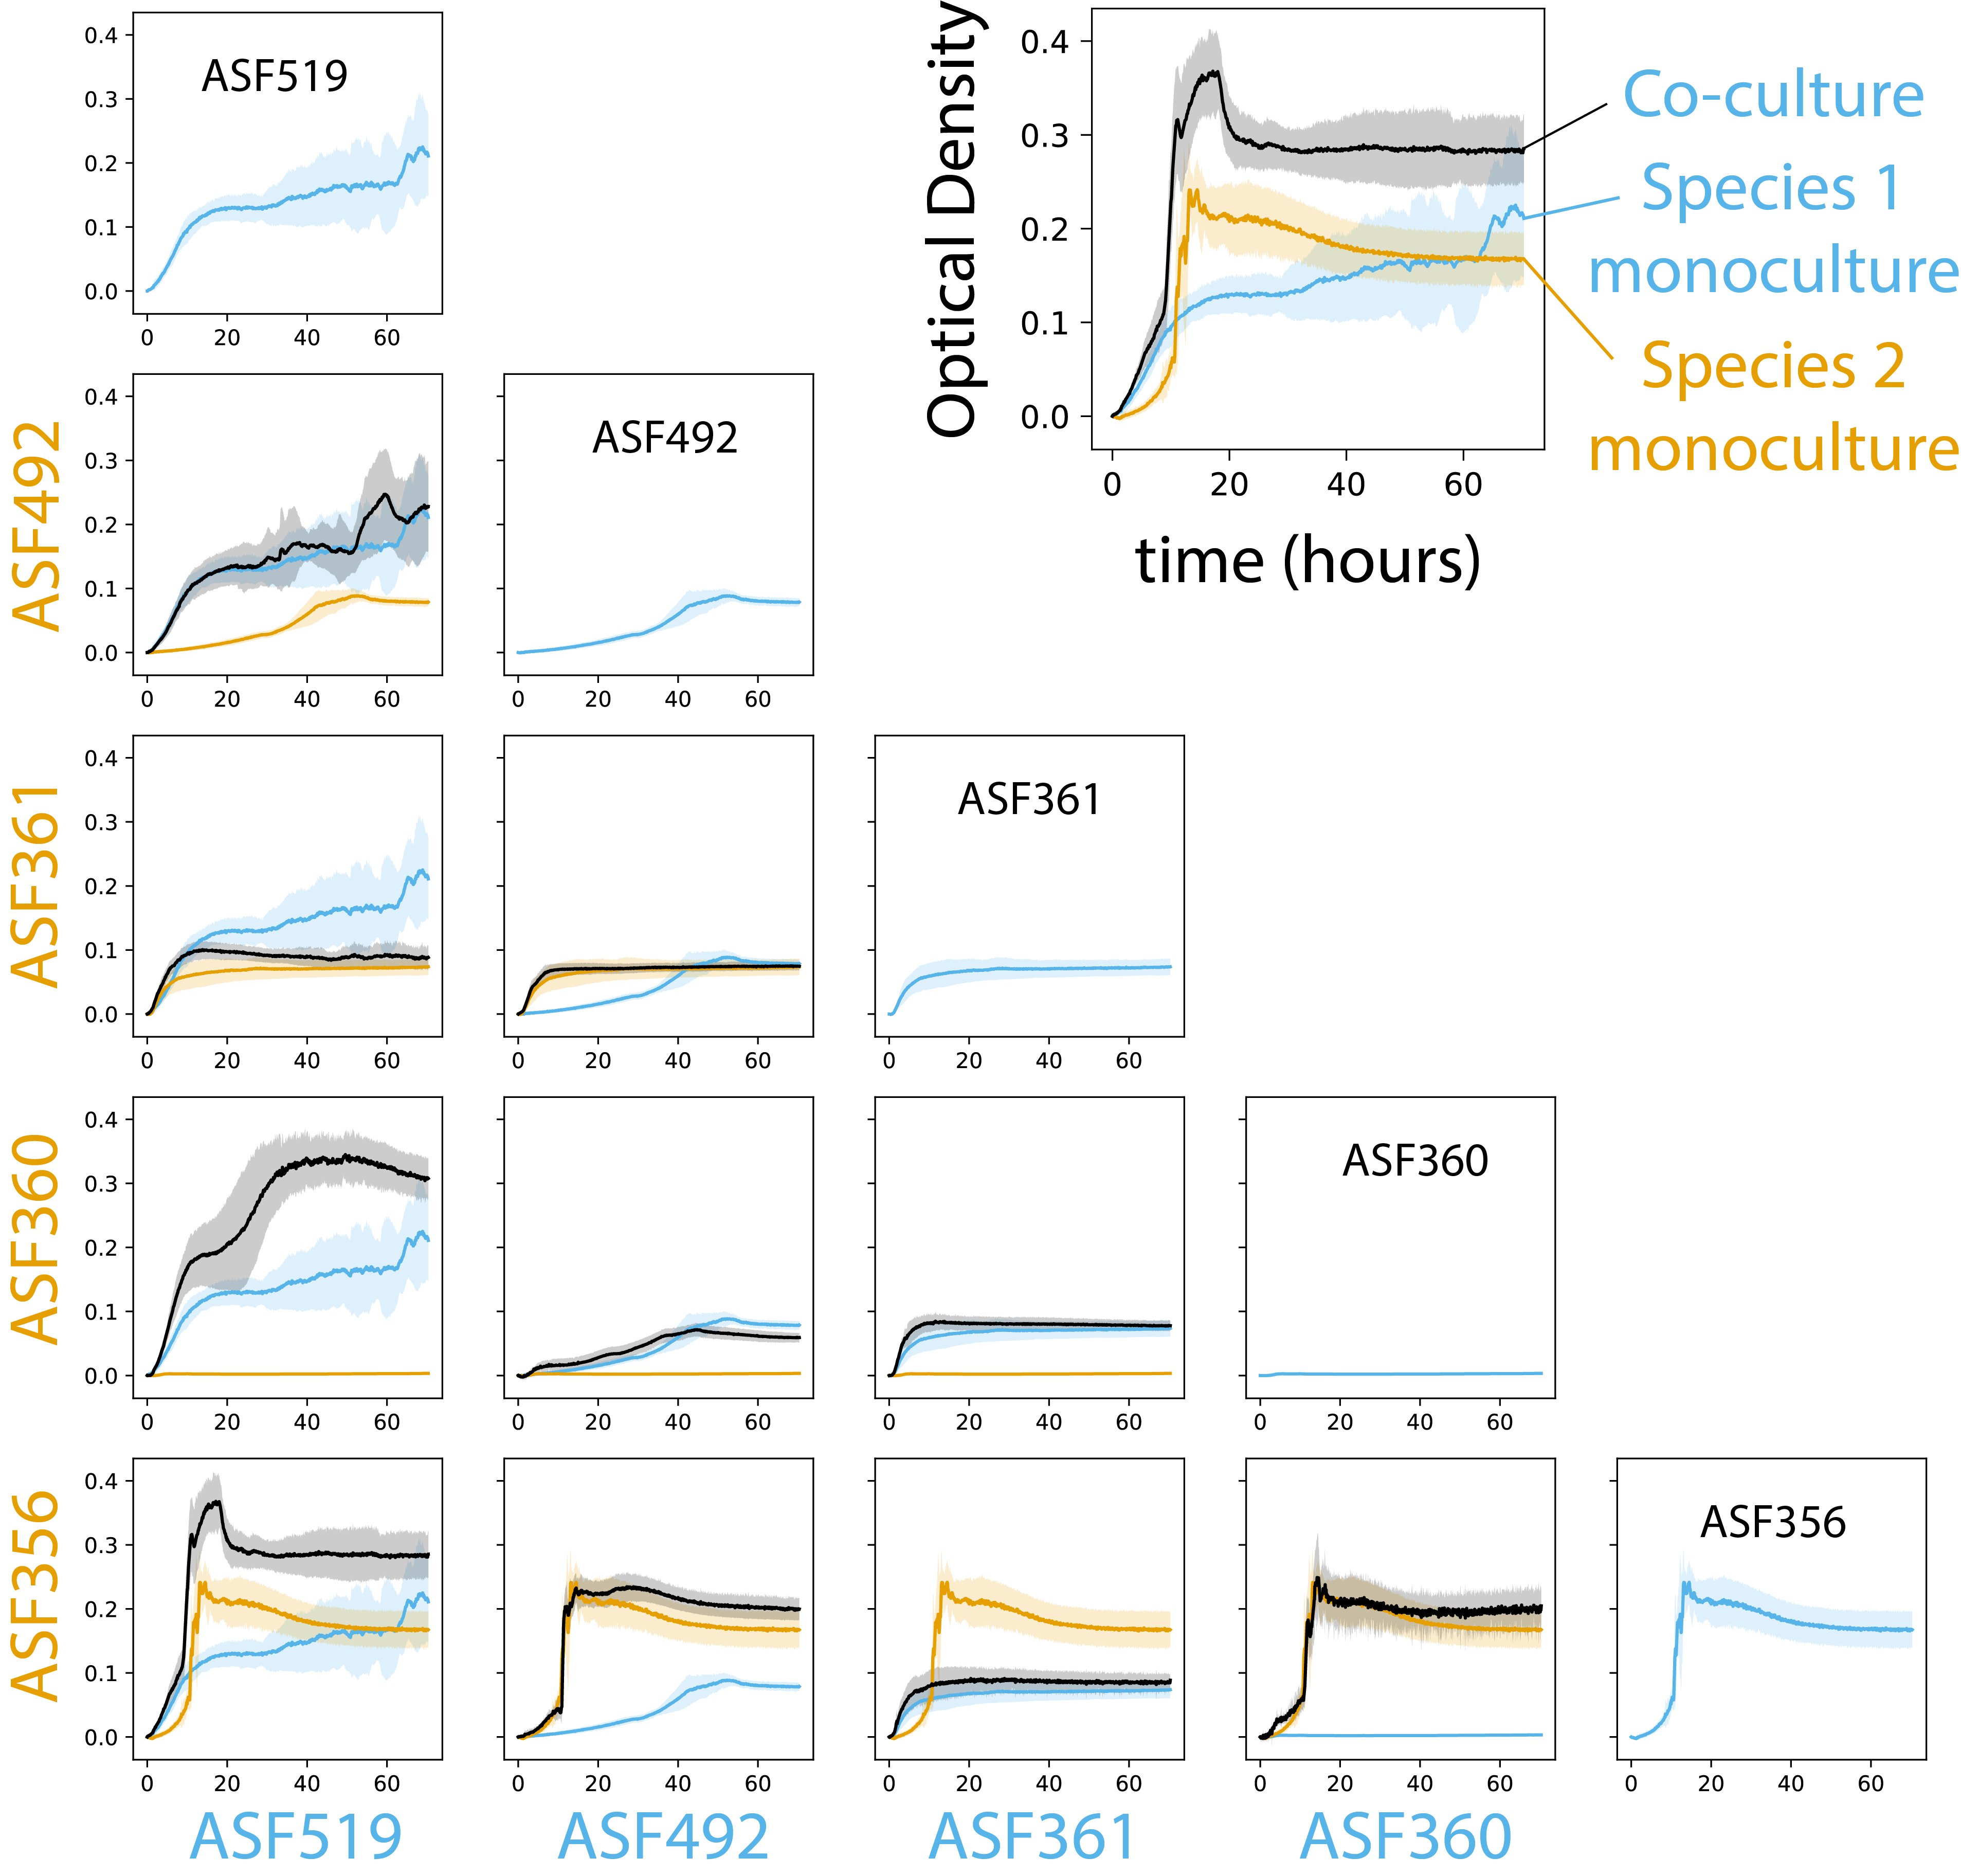
\includegraphics[width=0.8\textwidth]{ch2_figS2}
\caption[Optical density-based growth curves for \textit{Clostridium} ASF356, \textit{Lactobacillus} ASF360, \textit{Lactobacillus} ASF361, \textit{Eubacterium} ASF492, and \textit{Parabacteroides} ASF519.]{\textbf{Optical density-based growth curves for \textit{Clostridium} ASF356, \textit{Lactobacillus} ASF360, \textit{Lactobacillus} ASF361, \textit{Eubacterium} ASF492, and \textit{Parabacteroides} ASF519.} Optical density was measured at 589nm. Experiments were performed in 96 well plates with 200uL total volume in each well. Each sample group (monocultures and co-cultures) contains 8 biological replicates from a single experiment (e.g. each replicate was grown in an independent well, but they were derived from the same starter culture). Line shows the mean for each sample group, and shading extends one standard deviation from the mean in both the positive and negative direction. Sky blue line indicates monoculture for the strain labelled in sky blue along the x axis. Orange line indicates monoculture for the strain labelled in orange along the y axis. Black line indicates co-culture of the two strains. Diagonal shows the monoculture growth curve for each species. Axes units are identical on all subplots. Time is shown in hours, extending to 72 hours.}
\end{figure*}

\begin{figure*}
\centering
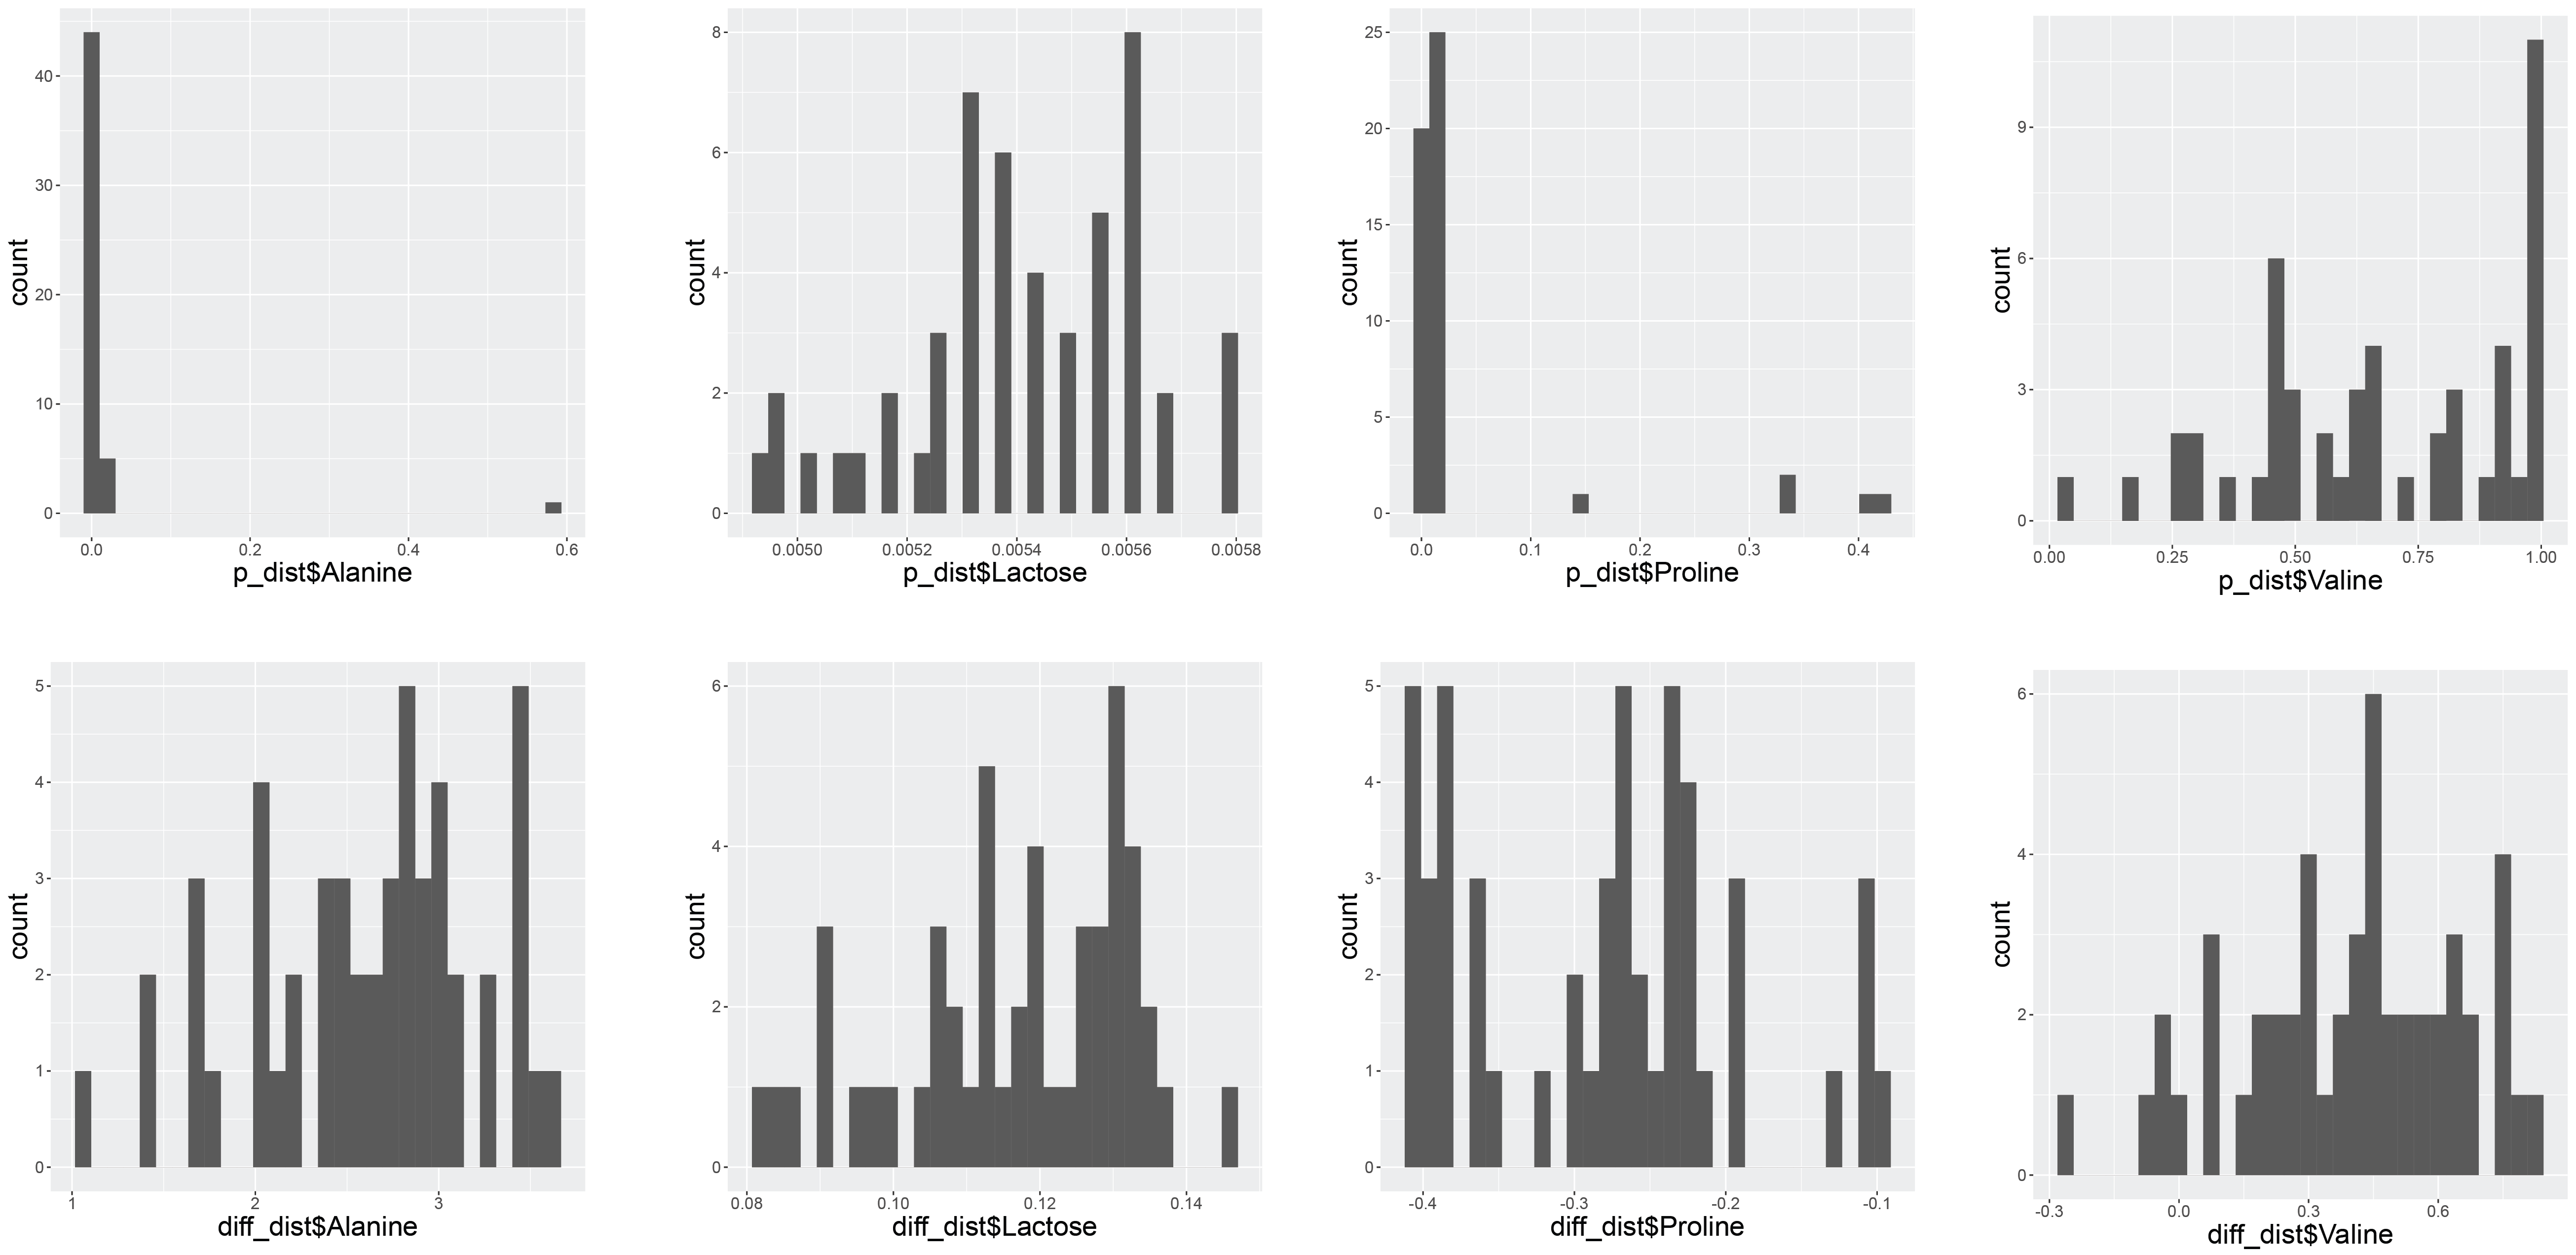
\includegraphics[width=0.8\textwidth]{ch2_figS4}
\caption[Selected examples of ConYE results using bootstrapped strain abundances.]{\textbf{Selected examples of ConYE results using bootstrapped strain abundances.} Top row shows the distribution of ConYE \textit{p}-values for each metabolite and bottom row shows the distribution of difference from the expected value for the same metabolite within each column. Examples are from the co-culture of \textit{Clostridium} ASF356 and \textit{Parabacteroides} ASF519. Distributions were generated by recalculating the average abundance of each strain in monoculture using leave-two-out bootstrapped samples prior to calculating the monoculture yield for each metabolite. N=50 samples with replacement for each monoculture.}
\end{figure*}

\end{refsection}


%------------------------------------------------------------------------------------
% Chapter 4 Reflections and Future Directions
%------------------------------------------------------------------------------------
\chapter{Reflections}
\begin{refsection}

\section{Reflections}

\section{Future Directions}

\section{References}

\printbibliography[heading=none]
\end{refsection}


\end{document}
